\documentclass[12pt]{report}
% Macro for http reference inclusion, per hypertex:
\def\href#1#2{\special{html:<a href="#1">}{#2}\special{html:</a>}}
\makeindex
\usepackage{times}

\usepackage[pdftex]{hyperref}
\usepackage[pdftex]{graphicx}

\begin{document}

\title{
\includegraphics{degas2d}
  Developer's Guide for DEGAS 2}

\begin{abstract}
  This document is an extension of the User's Manual
  and the inline documentation generated from the
  FWEB source files.  Its objective is to provide
  additional details on critical aspects of the code's
  operation that needed by future developers.
\end{abstract}

\maketitle

\chapter{Geometry}

\chapter{Scoring}

\section{Introduction}
The estimators in DEGAS 2 are calculated by
the routines in {\tt score.web}, which are invoked during tracking.
At the end of each flight, the resulting data are accumulated into the
global arrays described in the \href{classes.pdf#page.65}{statistics class} 
(package abbreviation {\tt sa}) via the subroutines in {\tt stat.web}.

The data accumulation process takes place over a range of scales
to optimize performance on massively parallel platforms.  The basic
breakdown is:
\begin{description}
  \item[flt] for ``flight''.  This always refers to a single flight.
  \item[frag] for ``fragment''.  To facilitate load balancing, 
only a fraction (or ``fragment'') 
of the total number of flights per processor
are sent at a time to each process.  
As each process completes, an additional fragment
is sent until all have been completed.
  \item[fin] for ``final''.  In the simplest case, this refers to
the global accumulation of data from all processes.  Again,
in the simplest case, the data are actually accumulated
directly in an array from the 
\href{classes.pdf#page.61}{output class}.
\end{description}

This process is complicated by two additional optimizations.
First, as is documented in the \href{classes.pdf#page.65}{statistics class},
these arrays may be compressed, especially at the {\tt flt} level,
to reduce the amount of data transmitted.  Second, in runs on
larger machines
(say, $> 100$ cores or processes) fragments are 
accumulated into intermediate ``final'' arrays over groups of
processors to reduce the number of accumulations that must
be performed by the master process, avoiding network 
transmission collisions. The machinery facilitating this is
contained in {\tt degasinit.web}.  

\section{Basic Expressions}
\label{expressions}
The sources of neutral particles to be simulated in a given
DEGAS 2 run are broken up into ``groups'' according to their
physical nature, e.g., ``plate recycling'', ``gas puff'', etc., 
as described in the \href{classes.pdf#page.26}{sources class}.  
Because the number of flights and total particle current
associated with each source group are specified independently
by the user, the data for each group are accumulated 
separately and are available by themselves within the
\href{classes.pdf#page.61}{output arrays}.

The fundamental expressions used in the data accumulation
process are, thus, for a specific source group $i$.  The 
other principal indexing parameters for the output arrays
are the geometric zones, $z$, and the tallies, as
contained in the \href{classes.pdf#page.52}{tally class}.
To minimize confusion, we do not introduce any explicit
index for the latter; the following expressions apply
independently for each tally.  The first accumulated moment,
to be associated with the mean in the end is:
\begin{equation}
S_{1}^{i}(z) = \sum_{j = 1}^{N_{i}} \rho_{j} \left (
\sum_{k \in z} \xi_{j,k} \right ) / \sum_{j = 1}^{N_{i}} \rho_{j},
\label{mean1}
\end{equation}
where: $i$ is the source group index, the ``1'' refers to the
first statistical moment, $j$ runs over all of the
$N_{i}$ flights in group $i$, $\rho_{j}$ is the relative
statistical weight of flight $j$, $k$ is the list of events
scored 
by flight $j$ (e.g., collisions) 
in zone $z$, and $\xi_{j,k}$ is the estimator
value (see below) 
for this tally recorded by flight $j$ during event $k$.
The statistical weight $\rho_{j} \equiv 1$ in most cases,
but can be set otherwise by the user to effect importance
sampling via the input arrays {\tt source\_segment\_rel\_wt}.
Note that this quantity is {\em fixed} for a given flight
(indeed, is the same for all flights launched from that
source segment) and is distinct from the statistical
weight [{\tt pt\_w(fl\_current(x))} in subroutine
{\tt follow}], designated by $w$ in the estimator expressions
below, which may
vary during flight tracking, but {\em always} has 
an initial value of $w = 1$.

Estimators are discussed in greater generality in the
User's Manual.  Here, we write out the ones of
greatest interest to provide adequate context
for the statistical moment expressions.
First, the estimator most commonly used in compiling
test particle data is the track length estimator, 
\begin{equation}
\xi_{g}^{\rm TLE} = w \, \frac{1 - \exp(-\sigma_{i} t_{V})}{\sigma_{i}} g,
\label{TLE}
\end{equation}
where  $t_{V}$ is the time the particle track spent in volume V,
$w =$ weight at start of the time step.  Note that in the
limit $\sigma_{i} t_{V} \ll 1$,
$[1 - \exp(-\sigma_{i} t_{V})]/\sigma_{i} \rightarrow t_{V}$,
so that estimator scales directly with the time spent in a zone.
For longer time intervals, e.g., as might be the case when other
reaction rates are small, 
the exponential factor effectively accounts for weight reduction
along the track.
The function $g$ can be a test particle attribute, such as
mass, momentum, energy, or reaction-related, e.g., ion 
momentum source due to charge exchange. Volumetric
plasma sources, such as the latter, 
enter the track-length estimator as averages over the background 
distribution.

The second type of estimator is the collision estimator,
\begin{equation}
\xi_{g}^{\rm CE} = \sum_{m_{s}} w_{m_{s}} 
\frac{g}{\sigma_{s}},
\label{ce}
\end{equation}
where the sum is over $m_{s}$, all scattering collisions within $V$,
and is equivalent to the $\sum_{k}$ in Eq.~(\ref{mean1}).
The quantity $w_{m_{s}}$ is the weight at $m_{s}$th collision.  If
suppressed absorption is being used, as is normally the case, the
particle weight will decrease between the collisions.
Again, $g$ is a test particle attribute.

There is an analogous expression for the collision estimator associated
with a particular reaction,
\begin{equation}
\xi_{g}^{\rm CE} = \sum_{m_{j}} w_{m_{j}} \frac{g}{\sigma_{j}},
\label{cereac}
\end{equation}
where the sum is now over $m_{j}$ collisions of reaction $j$ within $V$,
The function $g$ is some quantity related to the reaction and is likely
something known only at collisions. One example of such a quantity would
be the energy source due to H$_{2}$ dissociation (i.e., the energy
exchange is determined only once the product velocities have been 
determined).


The equivalent expression for the second moment is:

\begin{equation}
S_{2}^{i}(z) = \sum_{j = 1}^{N_{i}} \rho_{j} \left (
\sum_{k \in z} \xi_{j,k} \right )^{2} / \sum_{j = 1}^{N_{i}} \rho_{j}
- \left [ \sum_{j = 1}^{N_{i}} \rho_{j} \left (
\sum_{k \in z} \xi_{j,k} \right ) / \sum_{j = 1}^{N_{i}} \rho_{j} \right ]^{2}.
\label{var1}
\end{equation}
While this expression is very close to that for the
variance appearing in statistics textbooks, it is not
suitable for the multi-level data accumulation used by
DEGAS 2.  
How one would break up the sum in the
numerator of Eq.~(\ref{mean1}) into smaller
sets (fragments) of
flights $j$ is clear.  
To do likewise for the second moment, we need to instead
work with:
\begin{equation}
\sum_{j = 1}^{N_{i}} \rho_{j} \left (
\sum_{k \in z} \xi_{j,k} \right )^{2} / \sum_{j = 1}^{N_{i}} \rho_{j} 
= S_{2}^{i}(z) + 
\left [ \sum_{j = 1}^{N_{i}} \rho_{j} \left (
\sum_{k \in z} \xi_{j,k} \right ) / \sum_{j = 1}^{N_{i}} \rho_{j} \right ]^{2}.
\label{var2}
\end{equation}

\section{Accumulating Data}
\label{accdata}
We now motivate the specific expressions used to accumulate
data from an individual flight into a fragment, and a fragment
into a final total.
In the interest of clarity, 
we introduce some simplified notation:
$\sum_{j = 1}^{N_{i}} \rho_{j} \rightarrow w$,
$S_{1}^{i}(z) \rightarrow S_{1}$, and $S_{2}^{i}(z) \rightarrow S_{2}$.
The subscript $i$ in the following represents ``incremental'' data
(e.g., an individual flight), $b$ represents the ``base'' data
(e.g., the fragment containing data from earlier flights);
the result of the accumulation will be new base data, indicated
with a prime.
The familiar form for the first moment is:
\begin{equation}
S_{1b}^{\prime} = (w_{i} S_{1i} + w_{b} S_{1b}) / (w_{i} + w_{b}),
\label{mean2}
\end{equation}
with the new base weight being:
\begin{equation}
w_{b}^{\prime} = w_{i} + w_{b}.
\label{weight}
\end{equation}
But, the code actually uses an equivalent form to maximize
numerical accuracy:
\begin{equation}
S_{1b}^{\prime} = S_{1b} + (S_{1i} - S_{1b})\frac{w_{i}}{w_{i} + w_{b}}.
\label{mean3}
\end{equation}

The analogous expression following from Eq.~(\ref{var2}) is:
\begin{equation}
(S_{2b}^{\prime} + S_{1b}^{\prime 2} ) w_{b}^{\prime}
= (S_{2b} + S_{1b}^{2}) w_{b} 
+ (S_{2i} + S_{1i}^{2}) w_{i}.
\label{var3}
\end{equation}
Thus,
\begin{equation}
S_{2b}^{\prime} = [(S_{2b} + S_{1b}^{2}) w_{b} 
+ (S_{2i} + S_{1i}^{2}) w_{i} - S_{1b}^{\prime 2} w_{b}^{\prime} ] / w_{b}^{\prime}.
\label{var4}
\end{equation}
The equivalent form that is coded up in {\tt stat.web} is:
\begin{equation}
S_{2b}^{\prime} = [S_{2b} w_{b} + S_{2i} w_{i} 
+ (S_{1i} - S_{1b})(S_{1i} - S_{1b}^{\prime}) w_{i} ] / w_{b}^{\prime}.
\label{var5}
\end{equation}
The equivalence of Eqs.~(\ref{var4}) and (\ref{var5}) can be
demonstrated most readily by adding and subtracting 
$S_{1b}(S_{1i} - S_{1b}^{\prime}) w_{i}$ inside the square brackets of
Eq.~(\ref{var4}) and using Eq.~(\ref{mean2}) for $S_{1b}^{\prime}$.  
Again,
this form improves numerical accuracy, e.g., in the case
where $S_{1i} \simeq S_{1b}$.

To see this, consider two limiting cases.  First, look at the
one in which the increment is
much smaller than the base value:  $S_{1i} = \epsilon S_{1b}$, where
$\epsilon \ll 1$.  We insert this in Eqs.~(\ref{var4}) and
(\ref{var5}), and drop second order terms in $\epsilon$ relative to 
higher order terms (as if lost due to finite precision).  Note that
we expect $w_{i} \leq w_{b}$ in almost all cases.   
since the $S_{2}$ terms are the
same in these equations, we work only with the $S_{1}$ terms.  
So, the familiar arrangement yields:
\begin{eqnarray}
S_{1b}^{2} w_{b} + S_{1i}^{2} w_{i} - S_{1b}^{\prime 2} w_{b}^{\prime} & \quad & \\
&\rightarrow& S_{1b}^{2}(w_{b} + \epsilon^{2} w_{i}) 
- S_{1b}^{2}(w_{b} + \epsilon w_{i})^{2}/(w_{b}+w_{i}) \\
&=&  S_{1b}^{2} [ w_{b} + \epsilon^{2} w_{i} - \frac{w_{b}^{2}}{w_{i}+w_{b}}(1 
+ \epsilon \frac{w_{i}}{w_{b}})^{2}] \\
&\simeq& S_{1b}^{2} [w_{b} - \frac{w_{b}^{2}}{w_{i}+w_{b}} (1 
+ 2 \epsilon \frac{w_{i}}{w_{b}} )] \\
&=& S_{1b}^{2} \frac{w_{i} w_{b}}{w_{i} + w_{b}} (1 - 2 \epsilon).
\label{comp1t}
\end{eqnarray}

The equivalent terms from Eq.~(\ref{var5}):
\begin{eqnarray}
(S_{1i} - S_{1b})(S_{1i} - S_{1b}^{\prime}) w_{i} & \quad & \\
& \rightarrow & (\epsilon - 1) S_{1b} [\epsilon S_{1b}  
- S_{1b} \frac{w_{b}}{w_{i}+w_{b}}(1 + \epsilon \frac{w_{i}}{w_{b}}) ] \\
& = & S_{1b}^{2} \frac{w_{i} w_{b}}{w_{i} + w_{b}}(\epsilon - 1)^{2} \\
& \simeq & S_{1b}^{2} \frac{w_{i} w_{b}}{w_{i} + w_{b}} (1 - 2 \epsilon),
\label{comp1n}
\end{eqnarray}
i.e., the same as Eq.~(\ref{comp1t}).

However, if $S_{1i} = (1 + \epsilon) S_{1b}$,
\begin{eqnarray}
S_{1b}^{2} w_{b} + S_{1i}^{2} w_{i} - S_{1b}^{\prime 2} w_{b}^{\prime} & \quad & \\
&\rightarrow& S_{1b}^{2}[w_{b} + (1 + \epsilon)^{2} w_{i}] 
- S_{1b}^{2}(w_{i}+w_{b})(1 + \frac{\epsilon w_{i}}{w_{i}+w_{b}})^{2} \\
& \simeq & S_{1b}^{2} [ w_{b} + (1 + 2 \epsilon ) w_{i} - (w_{i}+w_{b})
(1 + \frac{2 \epsilon w_{i} }{w_{i} + w_{b}}) ] \\
& \rightarrow & 0!
\end{eqnarray}
But, with the modified form, 
\begin{eqnarray}
(S_{1i} - S_{1b})(S_{1i} - S_{1b}^{\prime}) w_{i} & \quad & \\
& \rightarrow & \epsilon S_{1b} [ (1 + \epsilon) S_{1b} - S_{1b}(1 
+ \frac{\epsilon w_{i}}{w_{i} + w_{b}})] w_{i} \\
& = & \epsilon^{2} S_{1b}^{2} w_{b} w_{i}.
\end{eqnarray}
That is, because $S_{1i} - S_{1b}$ appears in both Eqs.~(\ref{mean3})
and (\ref{var5}), the factors of $\epsilon$ enter via separate
terms, reducing round-off errors.

\section{Implementation in the Code}
\label{implementation}

The flexibility and generality of the scoring machinery in
DEGAS 2 can make relating the expressions in the previous
sections to the lines in the code challenging. 
Virtually all of the scoring in DEGAS 2 begins
in the tracking loop of subroutine {\tt follow}
with a
call to one of: {\tt score\_sources}, {\tt score\_reaction},
{\tt score\_test}, or {\tt score\_sector} (which invokes
{\tt score\_diagnostics}).
Note that {\tt score\_reaction} and
{\tt score\_sector} also serve as 
the
starting point for processing the corresponding action
indicated by its name.
This was also true of {\tt score\_sources} until the option
of sampling on the master processor was implemented.

For all of the scoring routines utilizing multiple estimator
types (i.e., all except {\tt score\_sector} /
{\tt score\_diagnostics}), the first argument is a
macro constant indicating the type of estimator to be
used for that call.  Note that {\tt score\_sources} is also called
with the post-processing estimator in subroutine
{\tt post\_process\_source\_scores}.

The routines {\tt score\_test} and {\tt score\_reaction}
compute the estimators described in Sec.~\ref{expressions}.
The second argument for these represents the time-like
quantity in Eqs.~(\ref{TLE}) - (\ref{cereac}).  In
particular, for the calls using the track length estimator,
{\tt tl\_est\_track}, the variable {\tt t\_fac} is
\begin{equation}
  t_{fac} = \frac{1 - \exp(-\sigma_{i} t_{V})}{\sigma_{i}}.
\end{equation}
For the calls with the collision estimator,
{\tt tl\_est\_collision}, the second argument is either
the inverse of the total scattering rate,
$\sigma_{s}$ ({\tt other\_rate} in the code), as in
Eq.~(\ref{ce}), or the rate of a single process,
$\sigma_{j}$ ({\tt rate[i]} in the code), as in
Eq.~(\ref{cereac}).

All of the argument lists for the scoring routines contain
an entry representing the current flight or, in the
case of {\tt score\_sector}, the entire flight stack.
In the latter case, the processing of the products of
plasma-material interactions (PMI) is handled in
{\tt score\_sector}, altering the flight stack.  This
is analogous what is done by the
collision estimator call to {\tt score\_reaction}
except that it returns the list of products (and reagents)
in the particle array, {\tt prod}, which is explicitly
processed in subroutine {\tt follow} into modifications
of the flight stack, {\tt fl\_pointer(x)} and
{\tt fl\_current(x)}.  In terms of scoring, the current
flight provides the weight factor, $w$,  in
Eqs.~(\ref{TLE}) - (\ref{cereac}).

All of the scoring routines also require the
{\tt estimator\_factors} argument, a 1-D array
with an entry for each of the tallies.  This
dynamic array is actually allocated in subroutine
{\tt do\_flights\_master} so that it can also be
used in the post-process scoring routines as well
as in the scoring routines called by subroutine {\tt follow}.
In the simplest cases of {\tt score\_sources} and
{\tt score\_diagnostics} (called by {\tt score\_sector}),
the nominal content of each entry in {\tt estimator\_factors} is
the weight of the current particle.
In {\tt score\_test} and {\tt score\_reaction}, this is
multiplied by the time-like quantity discussed
above and represented locally by the variable
{\tt est\_fac}.

The {\tt estimator\_factors} array also enforces the
estimator dependence of each tally contained in the
{\tt tally\_est\_test} and {\tt tally\_est\_reaction}
arrays for test and reaction / source scores, respectively.
These
arrays provide an overall $1$ ($0$) factor if
the current estimator is (is not) being used for a particular
test tally or reaction / source tally for a particular
reaction or source type (see the
\href{classes.pdf#page.52}{tally class}).
If all of the {\tt estimator\_factors}
for the current score type are zero, the local flag
{\tt need\_scores} will be set to {\tt false} and the
remainder of the scoring process will be bypassed.

Assuming that is not the case (i.e., {\tt need\_scores}
is {\tt true}), 
the quantities corresponding to $g$ in
Eqs.~(\ref{TLE}) - (\ref{cereac}) are computed; these
are stored in the local array {\tt scoring\_data}.
The length of this array is the macro constant
{\tt scoring\_data\_max}, defined as part of the
tally class in {\tt tally.hweb}.
The nominal content of {\tt scoring\_data}
is the set of dependent variables contained
in 
the \href{classes.pdf#page.84}{problem class}, i.e., the
macro parameters {\tt pr\_var\_mass}, etc.  A key
feature of this list is that it is extended as a part
of {\tt problemsetup}, e.g., to handle user-specified
emission lines, with the total number of entries being
given by {\tt pr\_var0\_num}.  During
{\tt tallysetup}, the assertion that
{\tt scoring\_data\_max} $>$ {\tt pr\_var0\_num} is
checked.  The specific reason that the length of
{\tt scoring\_data} is not set to {\tt pr\_var0\_num}
instead has been forgotten!

Subroutine {\tt test\_score} is the
simplest of the scoring routines.
The principal values of the variable
$g$, computed in 
subroutine {\tt test\_scoring\_data}, are the particle's
mass, momentum vector, and energy.  The
{\tt pr\_var\_xy\_stress} variable, $m v_{1} v_{2}$,
is also provided for use in the
\href{degas2_all.pdf#page.83}{Couette Flow example}.  Note
that additional elements of the stress tensor
could be compiled in the same manner, if needed for
a future application.

% Subroutines {\tt score\_diagnostics} and
% {\tt sector\_scoring\_data} have an analogous relationship.
% The code there is complicated first by the
% potential presence of two sectors at this zone boundary
% and second by the need to track mass, momentum, and
% energy both into and out of the sectors.  The call
% to {\tt sector\_scoring\_data} is inside
% {\tt score\_diagnostics'} main
% loop over the PMI ``products'' and is thus invoked
% for the incoming particle as well as any particles
% resulting from the PMI.  The orientation of
% each particle relative to the zone boundary is
% contained in the ``{\tt sector}'' and
% ``{\tt sector\_next}'' values carried by its
% \href{classes.pdf#page.11}{location class}.
% The handling of the of the orientation of the
% sectors and tallies is all dealt with in
% {\tt score\_diagnostics} via arrays from
% the sector and tally classes, as opposed to
% making such decisions in {\tt sector\_scoring\_data}.
% XXXX Thought about going into score_diagnostics in more
% detail here, but too many things to unravel, like
% sector_type_pointer and tally_geometry_ptr.  Am
% thinking to instead go into that as part of a
% tally related guide. - Have begun trying to do
% just this, hence, commenting out the above.

In subroutine {\tt score\_reaction}, the
task of filling the {\tt scoring\_data}
array is handled by the ``collision'' routines.
When a collision type estimator is being processed,
an actual collision routine, which results
in modifications to the flight stack,
is called via subroutine {\tt pick\_reaction}.
For track and post-processing estimators,
the track-length versions of the reaction
routines are invoked via subroutine
{\tt pick\_track\_reaction}.  These have
no impact on the characteristics of the
current flight; in fact, subroutine {\tt follow}
asserts that these calls to {\tt score\_reaction}
return no products.
All of these reaction routines provide
the entries in
{\tt scoring\_data} corresponding to 
the changes in ``problem
species'' (the union of the test and background
species lists) mass, momentum vector, and
energy.
For those processes that result in the emission
of photons, e.g., ionization
and dissociative excitation, values for
the emission rate and velocity vector of the
emitting species are included in the {\tt scoring\_data}
array.

Each of the source types has a corresponding
``data'' routine, e.g., subroutine
{\tt puff\_data}, that is called from
subroutine {\tt score\_sources} and fills in the
{\tt scoring\_data} mass,
momentum vector, and energy sources
for it. Subroutine {\tt plate\_data} handles
both the {\tt so\_plate} and {\tt so\_plt\_e\_bins}
types.  A recombination source is handled more
like a reaction, however, in that it provides
scoring data for multiple species and also results
in light emission.  To underscore this point, the
{\tt recombination\_data} subroutine is actually
kept in the {\tt collide.web} file.

\subsection{Sector and Diagnostic Scoring}

The scoring of sectors and diagnostics
in {\tt score\_sector} is
complicated first by the
presence of two sectors at a zone boundary
and second by the need to track mass, momentum, and
energy both into and out of the sectors.
The subroutine first sets {\tt sector1}
to {\tt lc\_sector} and {\tt sector2} to {\tt lc\_sector\_next} for the
current flight.  Their values will be used to determine if
the current flight is at an exit, in which case the current
flight is terminated immediately.  Or if it is at a wall / target
interface, in which case a PMI is processed. The comment after
the setting of {\tt sector1} and
{\tt sector2} described the objectives of the next three lines,
but understanding them is crucial to comprehending the subsequent
subroutine calls:

\begin{verbatim}
nprod = 0
\end{verbatim}
Anticipates the possibility of a purely diagnostic interface
in which no PMI or exit is processed; i.e., the current
flight goes on its way as is.

\begin{verbatim}
pt_copy(fl_current(x),prod[0])
\end{verbatim}
Both the {\tt process\_pmi} and {\tt score\_diagnostic}
subroutines operate on {\tt prod[0]} (and subsequent
elements in the case of a PMI), so it must be a copy
of the current flight particle.

\begin{verbatim}
pt_thru_face(fl_current(x))
\end{verbatim}
Again, this line anticipates the possibility of a purely
diagnostic interface.
The macro invokes {\tt lc\_thru\_face} in {\tt location.hweb},
which in turn sets {\tt lc\_cell} to {\tt lc\_cell\_next} and
likewise for {\tt lc\_sector} and {\tt lc\_sector\_next}.
As implied by its name, the macro effectively
puts the particle on the other side of the
interface.  If there is a PMI or the current flight
is at an exit, the flight is killed, and this macro
does not matter.  This has no impact on the scoring since
that is now going to be done on {\tt prod[0]}.

These lines are followed by a loop over the non-diagnostic
sectors; i.e., {\tt type} $=$ {\tt sc\_vacuum} $= 1 \rightarrow$
{\tt sc\_exit} $= 5$, which is also the value of
{\tt sc\_diagnostic(0)} (see the corresponding macro in the
\href{classes.pdf#page.39}{sector class}).
The way this loop is written amounts to
``overkill'' in that both ``{\tt sector}'' and
``{\tt sector\_next}'' are tested and that only three
of the five sector types (wall, target, and exit) result
in any action.  This structure harks back to earlier
incarnations of the ``sector'' concept.  In the wall and
target cases, the requisite PMI is processed.

The operation of PMI related routines is discussed
elsewhere (e.g., in the User's Manual sections on
\href{degas2_all.pdf#page.56}{Recycling} and
\href{degas2_all.pdf#page.112}{Adding Reactions and PMI}),
but noting a few details here will help clarify the
operation of sectors and diagnostics.  Note, first,
that the PMI yields may be functions of the test particle
incident angle, $\theta$, measured relative to the surface
normal, and $\cos(\theta)$.  The latter is provided by
the function {\tt intersection\_direction}, which in
turn invokes {\tt surface\_intersection\_direction}.
As is noted there, $\cos(\theta) > 0$ means the
particle is leaving that surface and cell.

The velocity of the PMI product is returned
by the PMI routines as if the particle were impinging on
the $X$ -- $Y$ plane.  When these routines return
the product particles to subroutine {\tt pick\_pmi},
the outgoing velocity vector is rotated into the proper
local orientation by subroutine {\tt surface\_reflect}.
This is then loaded into the velocity of the
{\tt prod} array of each product along with
the location of the incoming product.  However,
this only amounts to copying its location
in configuration space, $\vec{x}$, since
the next lines of code proceed to set the
{\tt lc\_cell} to the products to the incoming
{\tt lc\_cell\_next} and vice versa; the same is
done for the sector and zone values.  This swap
is explained in the comment: the scoring is
performed as if the incoming (outgoing)
particle is leaving (entering) the plasma or vacuum
zone and entering (leaving) the solid
zone.  Once control returns to subroutine
{\tt score\_sector}, {\tt score\_diagnostics}
is called.  Before delving into it, note that
upon its return, the {\tt pt\_thru\_face}
macro is called for each product so that each
is then labeled as being in a plasma or vacuum
zone (and cell) and is, thus, ready to be tracked.
The face and sector values
at this point are incorrect, but these
are not needed for tracking and
test or reaction scoring.

The values of the {\tt sector}
and {\tt sector\_next} for the current and
product particles when
{\tt score\_diagnostics} is called
are shown schematically in Fig.~\ref{pmisectors}.
An outer loop, {\tt j} $= 0 \rightarrow$ {\tt nprod},
cycles through each of the current and product
particles.  Inside of this is a loop over all
of the tallies of type sector, with tally
number {\tt jscore}.  Yet another loop
with index {\tt i\_side} considers the two
sides of the interface; as in Fig.~\ref{pmisectors},
the values of the local variable {\tt sector}
is set using either {\tt lc\_sector} or {\tt lc\_sector\_next},
likewise for the local variable {\tt zone}.

\begin{figure}
  \begin{center}
    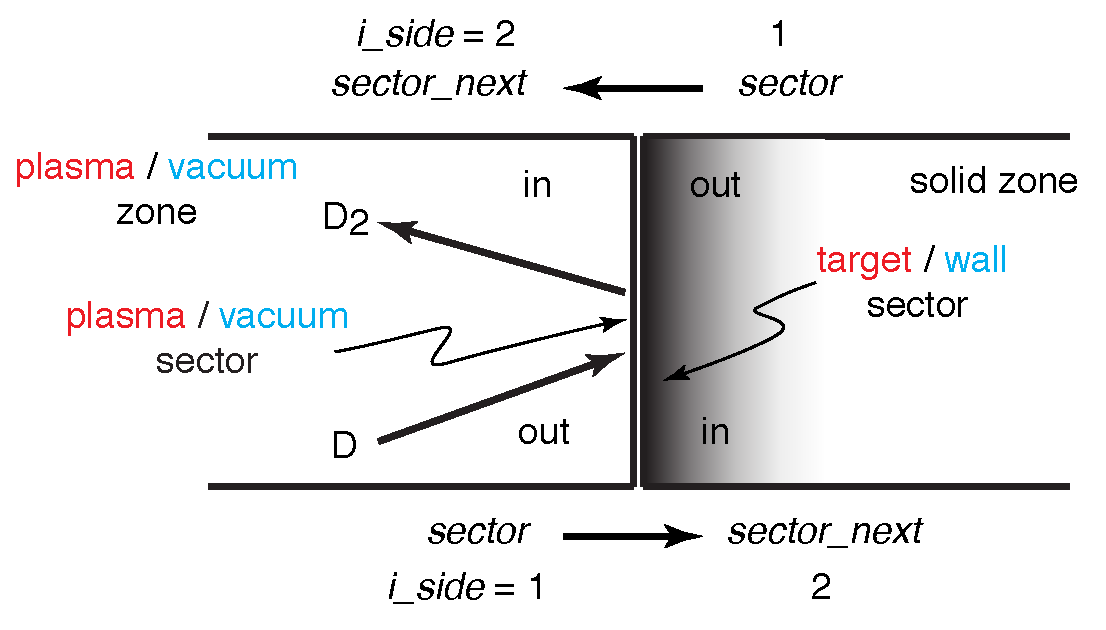
\includegraphics[width=4in]{pmi_sectors.pdf}
    \caption{Schematic for a desorption PMI showing
      the sector values used by subroutine
      {\tt score\_diagnostics}.}
    \label{pmisectors}
  \end{center}
\end{figure}
  
The {\tt surface} identifier corresponding to {\tt sector}
is obtained from the {\tt sector\_surface} array;
this is unique.  The number of sectors,
{\tt count},
associated with this surface then comes from
{\tt surface\_sectors}.  The value
of {\tt count} may be $> 1$ for two reasons.
First,
in 3-D cases 
a single surface may bound all of the zones
constructed from a discretization in the toroidal
direction.  However, only one of those will have
the same zone as the one being scored.  More
relevant in this case is that purely diagnostic
sectors may have been defined for this surface
and zone combination; see the description
of \href{definegeometry2d.pdf#page.18}{auxiliary
  sectors} in {\tt definegeometry2d} (note that
much of the above description of sectors, etc.
is echoed in its preamble and other documentation).

Because of this latter possibility, yet
another loop goes through each index of
the loop looking at one of these
sectors, sector number {\tt subsector}.
The key point of this set of nested loops
is to identify which tallies need to be
updated at the particle's location.  For
this to be the case, three conditions must
be satisfied:
\begin{enumerate}
\item The ``geometry operator'' for the
  tally {\tt jscore} (e.g., ``Wall and Target Counts'';
  see the \href{tallysetup.pdf#page.2}{tallysetup
    documentation}) must include one of the
  sectors {\tt subsector} associated with {\tt sector}.
\item The zone associated with
  {\tt subsector} is the same as the current {\tt zone} value.
\item The dependent variable for tally
  {\tt jscore} is consistent with the ``in'' / ``out''
  convention depicted in Fig.~\ref{pmisectors}.
\end{enumerate}
If these conditions are met, {\tt estimator\_factors[jscore]}
is set to the particle weight; if not, the value is left at
the default value of zero.  The last of these three is a
key point; this is where the directionality of the
diagnostics is enforced.  In principle, this could have
been done (and in earlier versions of the code, was done)
in the subsequent subroutines {\tt sector\_scoring\_data}
or {\tt handle\_diagnostics}.

At the completion of these loops, but still inside the
loop over the current and PMI product particles,
{\tt sector\_scoring\_data} is called to fill in
the {\tt scoring\_data} entries for angle, energy,
as well as the mass, momentum vector, and energy
in both the ``in'' and ``out'' directions.  These
are actually the same since, again,
the directionality is enforced in subroutine
{\tt score\_diagnostics}.

\subsection{Subroutine {\tt add\_scores}}

At the end of each of the main scoring routines,
such as {\tt score\_test}, is a call to subroutine
{\tt add\_scores}.  This is the point at which
the information from this step ({\tt score\_test}),
collision ({\tt score\_reaction}), sector
crossing ({\tt score\_sector}), or
source sampling ({\tt score\_sources}) gets added to
the {\tt stat\_flt} array that contains all
of the scores generated by the current flight.
Each invocation of {\tt add\_scores} is, thus,
for a particular type of tally: sector, test, or
reaction; this is the first argument for
{\tt add\_scores}.  The second argument is a
particle; this will be the current particle in the
case of {\tt score\_test}, {\tt score\_reaction},
and {\tt score\_sources}.  In {\tt score\_diagnostics},
{\tt add\_scores} is called separately for each
PMI product (if any; purely diagnostic sectors
have no products with {\tt nprod} $= 0$).
% The call to {\tt add\_scores} from subroutine
% {\tt score\_reaction} is not handled in this
% same way since the list of physical quantities
% inserted into the {\tt scoring\_data} array
% are the same (mass, momentum, and
% energy changes) for all of the ``problem species''
% involved in the reaction; their location
% in the {\tt scoring\_data} array is
% determined by their problem species number.
The third argument
is the problem reaction number; this is non-trivial
only for the calls by {\tt score\_reaction} and
{\tt score\_sources}.

The {\tt index\_parameters} array contains
the values of the tallys' independent variables.
The corresponding indices are set in the
\href{classes.pdf#page.59}{tally class};
see also subroutine {\tt set\_var\_list}
in {\tt tallysetup.web}.

The main loop in the subroutine is over all
tallies, {\tt jscore},
of the type specified by the first argument.
The first task performed in this loop
is a check to see if ``track conversions''
(see \href{classes.pdf#page.59}{tally class
  documentation} and
\href{tallysetup.pdf#page.3}{tallysetup})
are needed for {\tt jscore}.  Next comes
a test to see whether or not
the dependent variable for the score
{\tt jscore} is one
of the mass, momentum, or energy change
variables (from a ``collision'' reaction
or a PMI sector).
If it is, the
start and end points for a loop over problem
species are defined, otherwise, these are set to trivial
values.  In both cases, the {\tt check\_data}
variable is compiled from the corresponding
entries in the {\tt scoring\_data} array to
determine whether or not its contents are trivial.
If the latter or if the
{\tt estimator\_factors} value for
{\tt jscore} is zero, the current loop is exited,
potentially saving significant effort.

Should both the {\tt estimator\_factors} and
{\tt check\_data} values be non-trivial,
the geometric aspects of the score are sorted
out by subroutine {\tt handle\_geometry}
(see \href{classes.pdf#page.59}{tally class
  documentation}.  For volume tallies,
the value of {\tt number\_segments} is 1 on
return and the content of the {\tt segments}
array is just the zone number of the current
particle.  For reaction (sector) tallies,
{\tt handle\_detectors} ({\tt handle\_diagnostics})
is invoked to fill in these data, as well
as any associated ``binned'' data.

For detectors, the list of ``segments''
consists of the detector chords associated
with the tally {\tt jscore} (its
``geometry operator'' or ``geometry ponter'')
that have non-zero contributions from the
current zone.  If the emission spectrum is being
computed for the tally, the ``bins'' contain
that information.  Additional details on
this can be found elsewhere.

The analogous steps for the sector based
diagnostics are taken in {\tt handle\_diagnostics}.
The structure of this subroutine resembles
that of {\tt score\_diagnostics} in that
it again examines the sectors on the two
sides of the current interface.  As noted
above, the number of sectors to be scored
on one of those sides may be $> 1$
due to the specification of a non-default
diagnostic surface there.   If
no non-default diagnostic surfaces
have been defined, the returned
value of {\tt number\_segments} $= 1$.
Moreover, the associated sector will be part
of either a solid or exit zone since
that's the case for all default sectors.
One difference between {\tt score\_diagnostics}
and
{\tt handle\_diagnostics}
is that the latter is
focused on a single diagnostic group,
like ``Wall and Target Counts''; the
list of ``segments'' returned is of members
of that group.

Following the call to {\tt handle\_geometry},
{\tt add\_scores} loops over these segments
and their associated ``bins'', if any, and
sets a corresponding entry in the
{\tt index\_parameters} array.  A third
loop goes through all of the ``problem
species'', if needed for this score, and
setting the entry for each in
{\tt index\_parameters}; if
not needed, the loop is trivial.
One final loop then goes through each
of independent variables for the
score {\tt jscore} and sets its
entry in {\tt ind\_val} from the contents
of {\tt index\_parameters}.
Once these are all set, and,
if needed, ``track conversions'' applied,
{\tt set\_comp\_scores} is finally
called to update the local copy of the output
arrays.

\subsection{Subroutine {\tt set\_comp\_scores}}

The subroutine itself is relatively simple.
Only two arguments are needed: the new contribution
to the current score and its location in the
output array.  The latter is provided
by the {\tt out\_array\_index} macro
(see \href{classes.pdf#page.62}{output class
  documentation}), which is
constructed using {\tt tally\_base},
{\tt tally\_dep\_var\_dim}, and {\tt tally\_tab\_index}.
The new contribution, {\tt datum}, is the
relevant entry in the {\tt scoring\_data}
array multiplied by the {\tt geom\_mult}
value returned by {\tt handle\_geometry}
(generally is $= 1$ except for detector based
scores) and the value of {\tt estimator\_factors}
for {\tt jscore}.  The seemingly complex sequence
of macros needed to identify the entry in
{\tt scoring\_data} handles the dependence
on problem species and on the rank of the dependent
variable (for vector quantities, such as
``momentum change'').

For the case in which {\tt stat\_comp\_flt}
is {\tt false}, {\tt set\_comp\_scores}, updates
the relevant entry in the {\tt stat\_flt} array
and returns.  If compression at the flight level
is turned on, the default, the subroutine first
checks to see if an entry in the {\tt ifull}
slot of the output arrays has been made yet.
If so, that entry is updated using
the {\tt stat\_ptr2short\_flt} mapping
(see the \href{classes.pdf#page.65}{stat class
  documentation}).  If not, the size of
{\tt stat\_flt} array is incremented,
the array
reallocated if needed, and the pointer
arrays {\tt stat\_ptr2short\_flt}
and {\tt stat\_ptr2full\_flt} assigned.

The end result of all of the calls to 
{\tt score\_test},
etc. for this flight as it is tracked through
subroutine {\tt follow} is effectively the quantity
$S_{1}$ discussed in Sec.~\ref{accdata}.

\subsection{Post Processed Scores}

For reaction type tallies, the user has the option
of scoring specific reactions after all of the flights
have been run and all of the data have been accumulated.
This process is initiated in a section of code near
the end of subroutine {\tt do\_flights\_master}
(in {\tt doflights.web}).  The code first checks to
see if any of the reaction type tallies
use the ``post processing'' estimator,
{\tt tl\_est\_post\_process}; if so, the
logical variable {\tt need\_scores} is set
to {\tt true}.  This is followed by a loop
over source groups.  The ``post'' and ``output''
final conversions (see \href{classes.pdf#page.57}{tally class
  documentation} and \href{tallysetup.pdf#1}{tallysetup documentation})
are applied in this loop;
these are performed even if {\tt need\_scores} is
{\tt false}.

If {\tt need\_scores} is {\tt true}, the subroutines
{\tt post\_process\_test\_scores} and {\tt post\_process\_source\_scores}
are called for each source group.  The only arguments to the
subroutines are the source group number and the
same {\tt estimator\_factors} array introduced earlier in
Sec.~\ref{implementation}.

The basic idea behind {\tt post\_process\_test\_scores}
is that we create a fake particle (i.e., an instance
of the particle class) having the location of each zone in
the problem space and weight equal to the number of
particles in that zone accumulated during the main
run.  Because the plasma parameters are constant
throughout that zone, all of the reaction rates are the same
for these particles.  For some scores, such as ionization
and light emission rates, the resulting tallies will
be the same as those obtained with a track length
estimator.

In the original implementation, the ``divide number''
conversion was used to transform the neutral flux into
an average particle velocity that could be used in this
same way to obtain post-processed tallies of momentum sources.
However, that conversion was found to give incorrect
results in runs with multiple source groups.  For this
reason, an arbitrary velocity vector is used, rendering
these post-process tallies incorrect.  The same is
true for energy source tallies.  Note that even if
``divide number'' worked as intended, additional code
would be required to correctly post-process energy source
tallies since the particle class does not have an ``energy''
property that could be used to transmit the average
particle energy in the cell to the reaction scoring routines.

Post-processing is nonetheless useful for some applications.
One example is the ``fixed neutral density'' approach
to computed a synthetic GPI diagnostic.  That fixed
neutral density is obtained via a normal run of the
code, using a track-length estimator 
with a particular plasma background.
Subsequent plasma time steps are then run as restarts
of DEGAS 2 based on the output file from that
initial run, but having the same number of
flights.  Since the number of flights is unchanged,
the main loop of the code does nothing.  By
changing the scoring of the reactions for the light
emission related tallies from track-length or collision
to post-process, the light emission rates are re-evaluated
with the new plasma parameters, effectively using the
same neutral density.  These restart simulations
take vastly much less time than the original.

The actual implementation in {\tt post\_process\_test\_scores}
is, in hindsight, needlessly general.  For example,
the particle number (and neutral flux vector) tally
has had only zone number and test species as the independent
variables in virtually every known run of the code so that
the explicit loops over all five ({\tt tl\_rank\_max})
possible independent variables is overkill.  The only
other less-than-obvious aspect of the code is indicated
by the existing comment noting that using the
{\tt lc\_set\_a} macro to set the particle location is
potentially time consuming and unnecessary.

The post-processing of source scores is more straightforward
in that they are based on the underlying kinetic distributions.
Note that a post-processing option has not yet been set up for
snapshot sources.  Doing so is possible, in principle, and
may be advantageous in that the resulting sampling of the
snapshot distribution might be more thorough (and, thus, more
accurate) than that obtained at run time.
Subroutine {\tt post\_process\_source\_scores} loops over
all segments, {\tt seg}, of the current source group.
The
corresponding {\tt kseg} $=$ {\tt seg} $-1$ and {\tt xseg}
(pointer to a geometry element, such as a sector or zone)
parameters are, thus, easily obtained from the segment number.
Just as with  a post-processed test score,
a fake particle is defined
for the scoring process with weight equal to the
source current at segment {\tt seg}.
The fake particle's location is intended to
approximate the average 
obtained by {\tt set\_source\_x} 
in run time sampling.
For surface sources, the midpoint
of the line segment is used; for volume sources, it's the zone
center.  The fake particle's velocity is non-zero only in the
case of a recombination source.   In the other cases, the
source sampling process does not depend on this velocity
so that it can be safely set to zero.   The fake particle
is then turned into a fake flight and passed on to the
{\tt score\_sources} subroutine.

This subroutine works in exactly the same way as during
run time.  The distinction arises only in the
subroutine calls that set up the ``data''
for each source type; in each case, the values
of sampled parameters are replaced by their averages.
For example, in the 
case of a plate source (subroutine {\tt plate\_data}),
the parameter
{\tt wa} $= 3$; in run time, this is
the square of the
unscaled velocity vector obtained by sampling from
a Gaussian distribution in each of the three spatial
directions (via {\tt rn\_gauss\_next}).  The parameter
{\tt vpuff} serves this exact same purpose in
subroutine {\tt puff\_data}.  In this case, one also
needs the average velocity vector as sampled from a
cosine distribution, which is $(0, 0, 8/3 \sqrt{6 \pi})$.
Note that this is correct only in the default case
of a pure cosine distribution; the more general ``cosine
to an exponent'' case is not handled.
For a plate source with a specified energy distribution,
subroutine {\tt plt\_e\_bins\_v\_details} uses the input
parameter {\tt wa} (in call from {\tt plate\_data}) /
{\tt urd} (its argument list) as a switch, with a value
of the macro {\tt real\_unused} telling it to compute
the average energy from the user specified energy
distribution.

For the volume source, the user specifies the
source's average velocity, $\vec{v}_{\rm src}$, and
temperature, $T$.  The
former becomes the fake particle's velocity.
Its energy is then just $1.5 T + 0.5 m v_{\rm src}^{2}$.

Scoring the recombination source is more complex due to
the associated light emission and electron energy losses
and sinks.  The fake particle's velocity is set from
the recombining ion's flow velocity in
{\tt post\_process\_source\_scores}.  In
subroutine {\tt recombination\_data}, the electron
energy source and loss rates are evaluated, as are the
wavelength and emission rate of the diagnostic lines
being simulated.  The ion energy lost is the thermal
value analogous to that shown above for the volume source.
The flow velocity vector and magnitude are loaded into
dedicated ``Maxwellian emitter'' slots in the
{\tt scoring\_data} array.  When {\tt add\_scores}
is called at the end of {\tt score\_sources} and it
in turn calls {\tt handle\_detectors}, these data are
used to compute the corresponding full emission spectrum.
This provides an enormous improvement in signal quality
over a collision-based score, making this another
very useful application of post-processed scoring.













% Note the comment in doflights.web: "we could have chosen to
% pass stat_flt by common".  Isn't that what we are doing?
% Revise accordingly.









\section{Final Processing}
\label{final}
The expressions in Sec.~\ref{accdata}
above are incorporated into subroutine {\tt stat\_acc},
although their equivalence is difficult to discern due to the 
bookkeeping associated with the compression of the $S$ arrays.
This routine is called at various points during the run to 
first accumulate ``flight'' data into a ``fragment''
array, and then the ``fragments'' into the ``final'' array.
The end result of this process is the 
{\tt output\_grp} array via the 
call to {\tt stat\_acc} in the ``Merge results'' macro invoked
by subroutine {\tt do\_flights\_master}.

As will be shown in more detail below, the 
mean tally values for each source group are scaled by the
total current in that group, which is obtained by summing
over the group's $N_{{\rm seg},i}$ segments:
\begin{equation}
\Gamma_{i} = \sum_{\ell = 1}^{N_{\rm seg},i} \Gamma_{i,\ell}.
\end{equation}
In the steady state 
mode of operation, $\Gamma_{i}$ represents a number of 
particles per second; in the time dependent mode,
$\Gamma_{i}$ is a number of particles.  Obviously, these
quantities are used in combining the $S_{1}^{i}(z)$ and
$S_{2}^{i}(z)$ over source groups.  But, they are also
used to scale the user-specified relative statistical
weights to get the $\rho_{j}$ appearing in 
Eq.~(\ref{mean1}), etc. above and in setting the
probabilities for sampling flights from the source
segments. 

Namely, the user can specify
an arbitrary 
set of relative weights, $r_{i,\ell}$, for segments $\ell =
1 \rightarrow N_{{\rm seg}, i}$ in group $i$.  
A normalization factor is computed for each source group:
\begin{equation}
r_{{\rm norm}, i} = \left ( \sum_{\ell = 1}^{N_{{\rm seg}, i}} 
\Gamma_{i,\ell} / r_{i,\ell} \right ) / 
\left ( \sum_{\ell = 1}^{N_{{\rm seg}, i}} 
\Gamma_{i,\ell} \right ).
\label{wtnorm}
\end{equation}
The cumulative probability distribution used in sampling flights
in group $i$ is, e.g., for segment $\ell$:
\begin{equation}
p_{i, \ell} = \left ( \sum_{m=1}^{\ell -1} \Gamma_{i,m} / r_{i, \ell} \right )
/  \left ( \sum_{m=1}^{N_{{\rm seg},i}} \Gamma_{i,m} / r_{i, \ell} \right ).
\label{cumul}
\end{equation}
These probabilities are computed without the weight
normalization factor Eq.~(\ref{wtnorm}) since it
would appear in both numerator and denominator.
The actual sampling procedure is more complex
and offers additional flexibility; see
the \href{classes.pdf#26}{sources class} and
\href{sourcetest.pdf}{sourcetest}.

If flight $j$ in group $i$ is sampled from 
segment $i$, the relative weight
is set to:
\begin{equation}
  \rho_{j} = r_{i, \ell} \times r_{{\rm norm}, i}.
\label{statwt}
\end{equation}

Scaling and final processing of the output arrays
is carried out by a couple of loops and subroutine
calls near the end of subroutine 
{\tt do\_flights\_master}.  In the first of the loops,
the means and variances are scaled by the relative
source currents:
\begin{equation}
P_{1}^{i}(z) = \frac{\Gamma_{i}}{\sum_{i} \Gamma_{i}} S_{1}^{i}(z)
\label{scaledmean}
\end{equation}
and
\begin{equation}
P_{2}^{i}(z) = \left( \frac{\Gamma_{i}}{\sum_{i} \Gamma_{i}} \right)^{2}
\frac{S_{2}^{i}(z)}{\left( \sum_{j = 1}^{N_{i}} \rho_{j} - 1 \right)}.
\label{scaledvar}
\end{equation}

At this point, $S$ represents {\tt output\_grp}, and $P$
represents {\tt out\_post\_grp}; the latter is also summed
over source groups to obtain {\tt output\_all}.

A second set of loops performs a final scaling
by the global total current, $\sum_{i} \Gamma_{i}$,
and a division by the time
interval  for time dependent runs.  The latter transforms the input
``current'' from a number of particles into an
average number of particles per second; in the interest
of clarity we do not explicitly show this factor
here.  At this stage, the variance is transformed
into the relative standard deviation that is used
externally to quantify the accuracy of the code's
results:

\begin{equation}
P_{2}^{\prime i} = \frac{( P_{2}^{i} )^{1/2}}{P_{1}^{1}},
\label{finalrsd}
\end{equation}
and 
\begin{equation}
P_{1}^{\prime i} = (\sum_{i} \Gamma_{i}) S_{1}^{i}
\label{finalmean}
\end{equation}



% The final estimated value for a given tally in 
% zone $z$ is, for each individual group:
% \begin{equation}
% E^{i}(z) = \Gamma_{i} S_{1}^{i}(z)
% \end{equation}
% In a time dependent run, this is divided by
% the simulated time interval $\Delta t = t_{f} - t_{i}$
% so that the dimensions are the same as in a steady
% state run.  This is then summed over all 
% groups to get the total:
% \begin{equation}
% E(z) = \sum_{i=1}^{N_{\rm groups}} E^{i}(z).
% \end{equation}

Namely, the expected
error in a statistical estimate of the mean $\mu$
via $N$ samples is $\sigma / \sqrt{N}$, where
$\sigma$ is the standard deviation and $\sigma^{2}$ 
is the variance.  
The relative standard deviation ``rsd'' is then
\begin{equation}
{\rm rsd} = \frac{\sigma}{\mu \sqrt{N}}.
\label{rsd}
\end{equation}

Note that Eq.~(\ref{var1}) and so on have 
$N \leftrightarrow \sum \rho_{j}$ in the denominator
of the variance even though $N-1$
appears in most textbook expressions.
The ``-1'' accounts for the fact that the 
same sample is used to estimate the mean $\mu$ and the variance.
While $N \gg 1$ in most DEGAS 2 runs, rendering the difference
between $N$ and $N-1$ negligible, retaining $N-1$
yields a maximum relative standard deviation of exactly
unity when $\rho_{j} \equiv 1$
(a single score; see below), facilitating interpretation of 
results.  In the process of computing the relative
standard deviation, we effectively multiply the 
$S_{2}$ by $N/(N-1)$.  The $N-1$ part of this is the denominator
in Eq.~(\ref{scaledvar}); the $N$ ends up being cancelled by the
$1/\sqrt{N}$ in Eq.~(\ref{rsd}) and does not explicitly
appear in Eq.~(\ref{finalrsd}).

The $P^{\prime i}_{1}$ and $P^{\prime i}_{2}$ quantities in 
Eqs.~(\ref{finalrsd}) and (\ref{finalmean}) again end up
in the {\tt out\_post\_grp} array and the sum over source
groups in {\tt output\_all}.

For purposes of explication, we combine the expressions in
Eqs.~(\ref{scaledmean} - (\ref{finalmean}) into:
\begin{equation}
P_{1}^{\prime i} = \Gamma_{i} S_{1}^{i},
\label{finalmean}
\end{equation}
and
\begin{equation}
P_{2}^{\prime i} = \frac{ \left[ \Gamma_{i}^{2} S_{2}^{i} 
/ \left( \sum_{j = 1}^{N_{i}} \rho_{j} - 1 \right) \right]^{1/2}}
{\Gamma_{i} S_{1}^{i}}.
\label{finalrsd}
\end{equation}

Finally, post-processed tallies are added to 
the {\tt out\_post\_grp} array and the ``conversion''
factors are applied via calls to subroutine
{\tt final\_conversion}.  The mean values 
in this are array are summed over
groups to obtain the means in {\tt out\_post\_all}.
Since the effects of the post-processing tallies
on the variance are {\em not} accounted for, 
the rsd's from {\tt output\_all} are copied into the
``variance'' entry in {\tt out\_post\_all}.

\section{External Use of Output Arrays}

The principal output of the code is contained in the
mean values of the {\tt out\_post\_grp} and
{\tt out\_post\_all} arrays.  Invariably,
the relative standard deviations in these arrays
are used to characterize the uncertainty
in the results, although the inclusion of
post-processed tallies may render those 
values inaccurate.  To be safe, one should use
the rsd's from ``test'' tallies, which 
are not available for post-processed scoring,
to quantify the uncertainty in a simulation.

None of the
scaling factors and transformations described 
in Sec.~\ref{final} are ever applied to the
{\tt output\_grp} array since it is used 
as input to
restarted simulations. 

This fact is forms the basis for the
{\tt acc\_output} utility, which is
used to effectively average over a number 
of simulations.  A related application is to
simulate neutral transport in the
presence of a 
time varying plasma background (since
the background is always assumed fixed
in time during a given run of DEGAS 2). 

The {\tt acc\_output} utility is called
after each run with the name of a ``base'' 
output netCDF file specified as a command line argument.
On the first such call, this file is assumed to
not exist.  The output file specified in the
{\tt degas2.in} file is read in and its 
{\tt output\_grp} array is scaled by 
$\Gamma_{i}$ for the mean and $\Gamma_{i}^{2}$ for
the variance.  These source strengths are
read in from the corresponding background file.
The resulting array is written
into the {\tt output\_grp} array in the ``base''
file.  Other data appear in the ``base''
file at this point, although they are not used.

On subsequent calls, the {\tt output\_grp}
data in the {\tt degas2.in} output file are again read
in and scaled by the source strengths.  The latter
come from the current background netCDF file;
this is an important consideration in that
they may differ from those of the previous run in
a time dependent application.  At this point,
the code invokes expressions Eq.~(\ref{weight}),
(\ref{mean3}), and (\ref{var5}), just as
in the {\tt stat\_acc} routine; these results
are placed in the {\tt output\_grp} routine of
the ``base'' file, facilitating successive
repetitions of this process.

With these data now representing a non-trivial
product of the input data, expressions 
equivalent to Eqs.~(\ref{finalmean}) and
(\ref{finalrsd}) are applied and inserted
into {\tt out\_post\_grp}; these are summed over groups
to fill {\tt output\_all}.  
By design, the $\Gamma_{i}$ factors have
already been applied.  Because the 
background plasma data may be different in the
constituent simulations, post-processed tallies
cannot be handled; the code will throw an
assertion if any are present.  The conversions
performed by subroutine {\tt final\_conversions}
{\em are} applied, yielding {\tt out\_post\_grp}
and {\tt out\_post\_all}.  Due to the exclusion
of post-processed tallies, the variances of 
both sets of output will be accurate.  The
resulting ``base'' file
can then be used just like a normal output file
in conjunction with {\tt outputbrowser},
{\tt geomtesta}, etc.  The two are not completely
equivalent since {\tt acc\_output} scales the 
{\tt output\_grp} array and does 
not update the {\tt output\_2D\_coupling} array 
(those data can be obtained directly from the 
 constituent tallies via {\tt outputbrowser}). 
The arrays {\tt output\_num\_flights} and {\tt output\_random\_seed}
are not utilized, either.  The total, accumulated
weight {\em is} available in {\tt output\_weight\_grp}.

\section{A Single Score}

In the special case of a single score
$\xi_{x}$ with weight $\rho_{x}$ in
a particular zone $x$, Eq.~(\ref{mean1})
simplifies to
\begin{equation}
S_{1} = \frac{\rho_{x} \xi_{x}}{\rho_{\rm tot}},
\end{equation}
with $\rho_{\rm tot} \equiv \sum_{j} \rho_{j}$.
Equation~(\ref{var1}) becomes
\begin{eqnarray}
S_{2} & = & \frac{\rho_{x} \xi_{x}^{2}}{\rho_{\rm tot}} 
- \frac{\rho_{x}^{2} \xi_{x}^{2}}{\rho_{\rm tot}^{2}}  \\
& = &\xi_{x}^{2} \frac{\rho_{x}}{\rho_{\rm tot}} \left ( 
\frac{ \rho_{\rm tot} - \rho_{x}}{\rho_{\rm tot}} \right )
\end{eqnarray}
Then, the relative standard deviation, which is 
effectively $\sqrt{S_{2}}/[\sqrt{(\rho_{\rm tot}-1)} S_{1}]$ 
reduces to:
\begin{equation}
{\rm rsd} = \frac{1}{\sqrt{\rho_{x}}} \left ( 
\frac{1 - \rho_{x}/\rho_{\rm tot}}{1 - 1/\rho_{\rm tot}} \right )^{1/2}.
\end{equation}
In the limit of $\rho_{\rm tot} \gg 1, \rho_{x}$, 
the ${\rm rsd} \rightarrow 
1 / \sqrt{\rho_{x}}$.  In the usual case of uniform weighting,
$\rho_{x} = 1$ and $\rho_{\rm tot} \rightarrow N$, ${\rm rsd} \equiv 1$,
as noted above.

Note, however, that when performing importance sampling, one can 
obtain single scores having $\rho_{x} < 1$ and, thus, an rsd $> 1$.
This is simply a reflection of that score carrying less than average 
statistical weight.  The rsd values in regions of the problem space
having adequate statistics can be interpreted via the same guidelines
as simulations with uniform weighting (e.g., as in Sec. 2.4 of the 
User's Manual).

\section{Handling of Relative Weights for Importance Sampling}

The path of the relative weight factors through the code, particularly
in the time dependent case, is sufficiently complex that it warrants
exposition.

\subsection{Setting up the source (e.g., in {\tt defineback})}

First, the relative
weights are stored in the array {\tt source\_segment\_rel\_wt}.
The default value of 1 is set 
in subroutine {\tt init\_wt\_alias} in {\tt writeback.web}.
Since importance sampling is rarely used, and schemes for employing it
must be adapted carefully to the problem at hand, no specific
code for it is provided; the user
is responsible for inserting code that will assign the desired values.
  
As an example, we provide a rough description of its
application to the time dependent version of the synthetic Gas Puff Imaging
diagnostic, where the objective is to ensure radially uniform
sampling of particles from the snapshot source.  For simplicity, the
relative weight computation is integrated into subroutine
{\tt set\_snapshot\_source}; the lines establishing the default values
in subroutine {\tt init\_wt\_alias} are then commented out.
In {\tt set\_snapshot\_source}, the problem 
space is divided up, somewhat arbitrarily,  into 1 cm radial bins, 
and the weights of the snapshot particles are
accumulated into them.  The total weight in each bin is then divided by the
global total to yield a fraction; this becomes the relative weight
factor associated with each bin and, thus, each snapshot particle
in that bin.  

As in the default version of subroutine {\tt set\_snapshot\_source}, the
{\tt source\_current} for each particle (i.e., each particle is a
``source segment'') is set to the snapshot particle's weight 
(without the relative weighting factor) and the total current,
{\tt so\_tot\_curr} for the source group.
The relative weight factors are then combined with the currents
in Eq.~(\ref{cumul}) to set up the sampling distribution.
The idea is that bins deeper into the plasma, where
penetration is poor, will have smaller relative weights.  This
will cause them to be preferentially sampled, as in Eq.~(\ref{cumul}).
An unbiased result is achieved by reducing the statistical
weight of these particles in the main code by the same 
relative weight factor.
The overall weight normalization factor,
{\tt so\_wt\_norm} is computed (by default) from the currents and relative 
weights via Eq.~(\ref{wtnorm}) in subroutine {\tt set\_prob\_alias}.

\subsection{Source sampling}

As is noted in {\tt sources.web}, subroutine {\tt sample\_sources},
the value of {\tt source\_segment\_rel\_wt}, scaled by
{\tt so\_wt\_norm}, is assigned {\em temporarily} to the sampled particle's
weight, {\tt pt\_w}.  In the {\tt ff\_copy} macro ({\tt flight\_frag.hweb}) 
invoked in
{\tt doflights.web}, subroutine {\tt setup\_flight\_frag},this scaled relative
weight is transferred into the {\tt ff\_float\_pt\_w} entry in the
{\tt ff\_particles\_float} array.

The associated {\tt ff\_label\_init} macro, also in {\tt flight\_frag.hweb},
returns this quantity as a macro parameter, {\tt rel\_wt}, and then sets
the flight's (instantaneous) statistical weight, {\tt pt\_w}, to 1.  
The overall weight of the flight, {\tt stat\_wt\_tot\_flt}, is equated
to that {\tt rel\_wt} parameter with the invocation of the
macro in {\tt flight.web},
subroutine {\tt do\_flights}; it is then globally accessible via the 
``stat'' ({\tt sa}) class and associated common blocks.  This is
the weight that is passed to subroutine {\tt stat\_acc} to accumulate
all of the scores from this flight and to obtain the total sampled
weight for the source group.  That is, the individual scoring routines,
such as {\tt score\_test}, record only {\tt pt\_w}.  However, when all of
those scores are combined with those from preceding flights, they are
effectively scaled by the relative weight factor via {\tt stat\_wt\_tot\_flt}.
Note that with importance sampling the
total weight in the source group is only 
approximately equal to the number of flights
sampled.

\subsection{Snapshot score and PDF}

Flights (in any source group)
reaching the end of the time step in time dependent runs
trigger a final call to {\tt score\_test} with the snapshot
estimator, {\tt tl\_est\_snaphshot}.  This will, obviously, lead
to the accumulation of data needed for tallying the snapshot density, etc.
But, it also results in a call to subroutine {\tt build\_snapshot\_pdf}
in {\tt score.web}.  The weight of the resulting entry in the
snapshot particle distribution function,
{\tt sn\_float\_pt\_w}, is recorded there as
the product of {\tt pt\_w} and {\tt stat\_wt\_tot\_flt}.  Once
all of the particles in a source group have been tracked,
the weights of the newly created snapshot particles are
scaled by the total current in the group, {\tt so\_tot\_curr}
(and the rarely used, arbitrary factor {\tt so\_scale}), and 
divided by the total weight in the group, {\tt output\_weigh\_grp}.
As noted above, in the subsequent time step, 
subroutine {\tt set\_snapshot\_source} ({\tt writeback.web})
sets the {\tt source\_current}
associated with this particle to the value of this {\tt sn\_float\_pt\_w}
entry in the snapshot arrays.

\chapter{Synthetic GPI Example}

\section{Introduction}

This document guides the user through an example
synthetic gas puff imaging (GPI)
simulation using XGC data.  Additional
details are provided to facilitate future applications.


\section{Geometry Setup}

\subsection{\tt efit2dg2d}
\label{efit2dg2d}

The triangular mesh used by XGC is too fine 
for this application, resulting in too long run times and /
or excessive Monte Carlo noise levels, as well as stressing memory
and storage resources.  We instead use the
{\tt efit2dg2d} routine to set up a triangular mesh over the
volume of interest.

The linear dimensions of the XGC mesh
triangles are roughly 1 mm.  The parameters in {\tt efit2dg2d}
and subsequently in {\tt definegeometry2d} are set so as
to result in triangles roughly three times this size,
significantly reducing computational requirements, but still
adequately resolving spatial variations in the XGC plasma
data.  Namely,
\begin{enumerate}
\item The box size and number of flux surface contours are
  chosen such that the average radial spacing between contours
  is roughly 3 mm. The resulting average spacing in $\psi$
  is about double that in the XGC mesh.
\item The outer edge of the contour box is taken to be 
  $R = 0.926$ m, large enough to yield continuous
  flux surfaces up to $\psi / \psi_{\rm sep} = 1.1$; the reason
  for doing so is described below.
\item The average poloidal spacing along the contours
  (the parameter {\tt r\_dtheta}) is 3 mm.
\item In {\tt definegeometry2d}, the area of the triangles
  around the gas nozzle is set to $5 \times 10^{-6}$
  m$^{2}$, close to the area of a 3 mm equilateral triangle.
\end{enumerate}

Given that the purpose of the synthetic GPI diagnostic is
to generate data suitable for validating XGC, our approach
is designed to use as much of the XGC simulation data as
is possible.  In the case of the application to Alcator
C-Mod, this entails altering the way that the split limiter
structure, which surrounds the GPI gas nozzles, is
incorporated into the simulation.  Given the relatively short
mean free paths of the atoms and molecules in the
vicinity of the plasma
facing surfaces of the limiter, the precise shape of those
surfaces is unlikely to impact the GPI light emission multiple
centimeters away.  Since those surfaces intersect the outer edge
of the XGC mesh and since both are nearly flux surfaces, we
opt to replace the limiter surface with a nearby flux surface;
the specific one is noted below.  The horizontal surfaces
of the limiter and the gas nozzle
are specified using engineering metrology
data.


The steps described here summarize the original procedure.
They would
need to be modified for a new application.

In {\tt efit2dg2d.web}, set the application macro:

\begin{verbatim}
@m APP CMOD_GPI
\end{verbatim}

Then, compile and run the code with the EFIT equilibrium for the
problem:

\begin{verbatim}
efit2dg2d XGC_GPI_19_ex/g1100223012.01149_261 
\end{verbatim}

As is noted in the preamble to {\tt efit2dg2d}, the spline
interpolation routine assumes that $\psi_{\rm sep} > \psi_{\rm axis}$.
This may not necessarily be the case in general, especially
for NSTX.  Should the spline routine generate an error, the
user should consult an EFIT expert for assistance in obtaining
a file compatible with this assumption.

\begin{itemize}
\item This yields a set of contours in the resulting
  {\tt wallfile}.
\item The corresponding set of polygons is in the
  {\tt polygons\_dg2d.in} file.
\item Both of these will be modified manually, as described in the 
    next step.
\item The {\tt stratum\_psi} file also produced relates the polygon
  stratum numbers to $\psi$ and radial coordinates.  This file
  is not used in this application since interpolation
      of plasma data is handled in a completely different way than
      in other {\tt efit2dg2d} applications, such as ENDD.
    \item The {\tt polygons.txt} file contains a
      point-by-point representation
      of the polygons in {\tt polygons\_dg2d.in} suitable for plotting;
      we will not be using this, either.
  \end{itemize}

\subsection{\tt definegeometry2d}
\label{definegeometry2d}

The construction of the 2-D input file to {\tt definegeometry2d},
{\tt xgc\_gpi\_19\_dg2d.in},
begins with the preamble.  The {\tt symmetry} is 
{\tt cylindrical}.
The $R$-$Z$ {\tt bounds} values are 5 cm outside those of the
box for {\tt efit2dg2d}, except for outer radial boundary.
The actual C-Mod vacuum
vessel is at $R = 1.0616$ m.  But, we set up these simulations
with it at $R = 0.98$ m to reduce the volume of the vacuum
region of the problem; this will be discussed in Sec.~\ref{statistics}
in connection with importance sampling.
However, still need to ensure that the camera vertex
at $R = 1.025$ m is in the universal cell; we do
this by 
setting the
outer radius of {\tt bounds} to $1.03$ m.
The {\tt wallfile} keyword points to a modified version of
the file produced by {\tt efitdg2d}, as will be explained
below.
Finally, the preamble section of the input file is terminated with
the {\tt end\_prep} keyword.

The next section of the input file consists of the polygons / strata,
1 through 34, extracted from {\tt polygons\_dg2d.in}.  The
polygons / strata 35 through 64 are deleted.
The full set of polygons described in {\tt xgc\_gpi\_19\_dg2d.in}
is depicted schematically in Fig.~\ref{polygons}.

\begin{figure}
  \begin{center}
    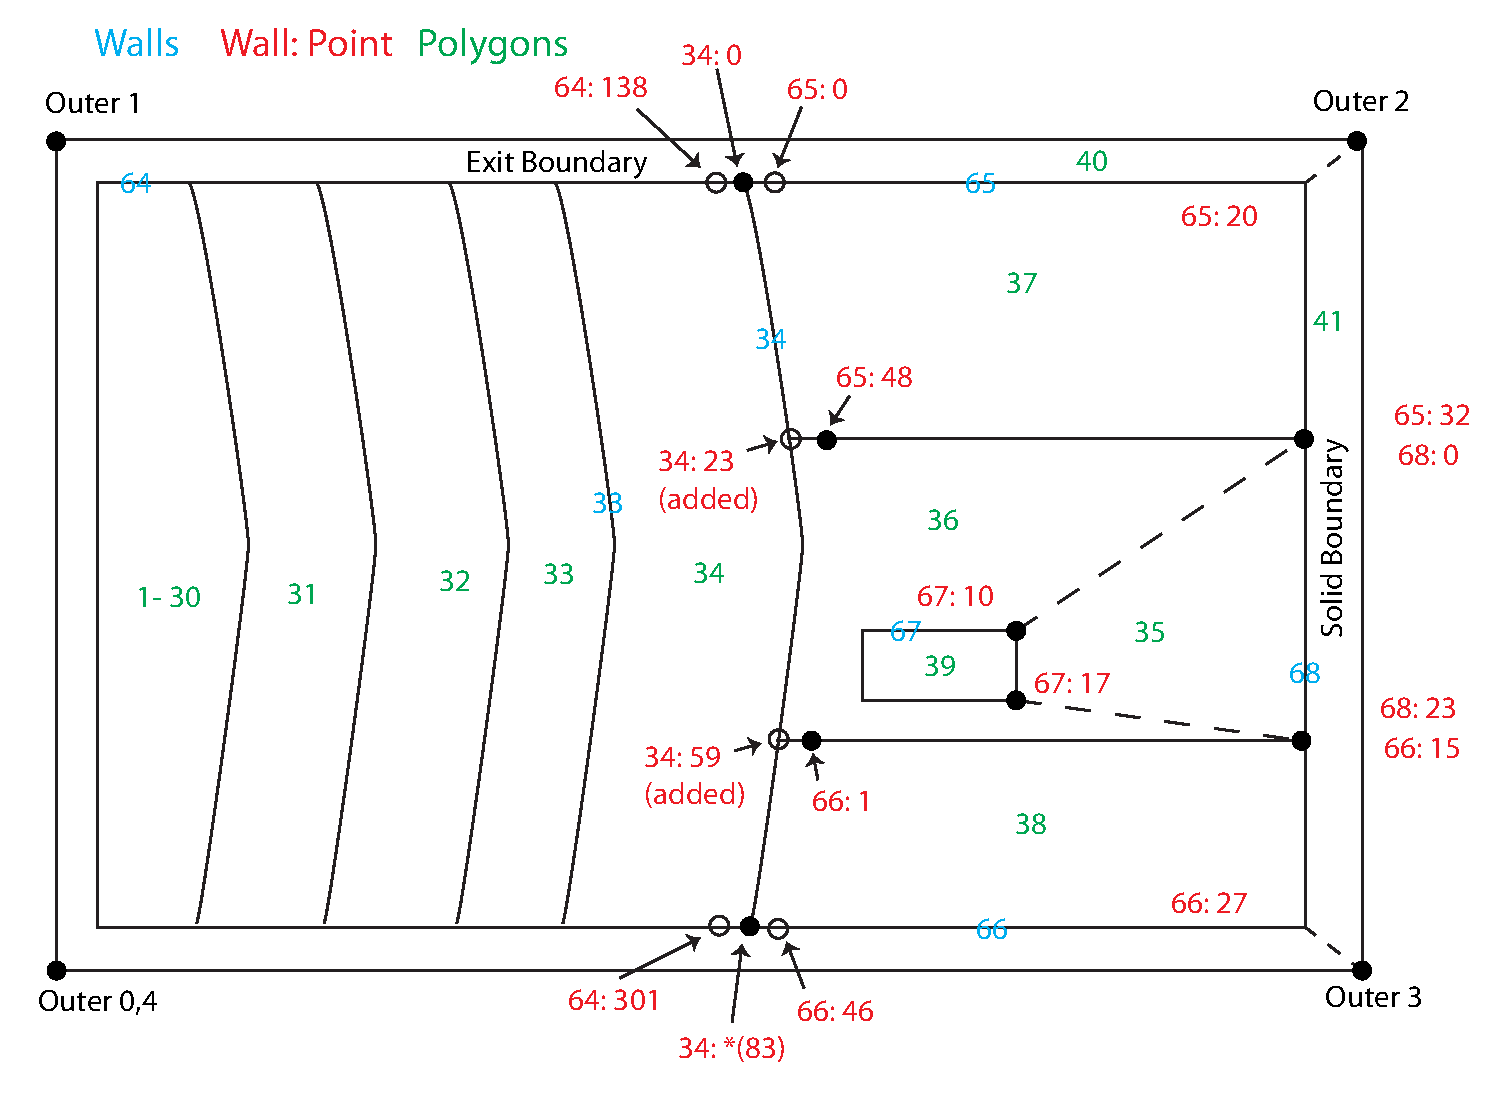
\includegraphics[width=4in]{alternative_geometry_19.pdf}
    \caption{Schematic depiction of polygons in the
      {\tt definegeometry2d} input file, {\tt xgc\_gpi\_19\_dg2d.in}.
      Polygon numbers are indicated in green; wall numbers in blue.
      Some key points are highlighted in red as (wall number):(point
      number).}
    \label{polygons}
  \end{center}
\end{figure}


To construct the remaining polygons, we need to modify and extend
the {\tt wallfile} produced by {\tt efit2dg2d}, resulting in
the {\tt wallfile.txt} pointed to by the {\tt wallfile} keyword.
Note that we do {\em not} delete the unused ``walls'' used in
the construction of strata 35 through 64 because
the last wall, wall 64, represents the complete outer boundary of
the contour box; reconstructing it from the other walls would be
possible, but extremely tedious.

We add four more walls to this file representing the upper and lower
limiter structures, the gas nozzle, and the section of the vessel
wall between the limiter structures.  These point lists were
created via a Python based script  used in constructing an earlier
version of this geometry.  Apart from their adherence to the
C-Mod metrology data the key characteristic of these point lists is
a roughly 5 mm spacing, consistent with the desired spatial resolution requirements
listed above.

One other change is to add two points to wall 34 where it meets up with
the limiter structures; the radial coordinates of these points is
determined by manual interpolation.  This change requires a corresponding
increment to the number of points at the top of the file. Note also
the insertion of the numbers of points in the four added walls.

The corresponding polygons are also manually constructed.   The most
important of these is stratum 36, labeled as ``Remaining volume around
nozzle'', since it is closest to the region of interest (the GPI camera
frame).  As noted above, we set the triangle area of this volume to $5
\times 10^{-6}$ m$^{2}$.  We do likewise for the ``Nozzle'' polygon,
stratum 39, since it contains plasma zones over most of the toroidal extent
of the problem.  The limiter halves and the volume behind the nozzle are
less interesting, so we increase the triangle area to $5 \times 10^{-5}$
m$^{2}$.  Note also that all of the solid polygons
are at the end of the file to allow the {\tt ucd\_plot} post-processor
to work as intended.





Before running {\tt definegeometry2d}, it must be compiled with the
{\tt detector\_setup} routine, contained in
{\tt cmodgpi\_camera4.web}, specifying the GPI and APD views.
Note that the GPI camera is located
at $\phi = 33^{\circ}$.  From your
run directory:

\begin{verbatim}
cp XGC_GPI_19_ex/cmodgpi_camera4.web ../src/usr2ddetector.web
gmake definegeometry2d
definegeometry2d XGC_GPI_19_ex/xgc_gpi_19_dg2d.in
\end{verbatim}

The end result of this process, apart from the obvious geometry
netCDF file, is a triangulation of the volume.  To facilitate
interpolation of the XGC data onto these triangles, we first
extract them from the polygon netCDF file produced by {\tt definegeometry2d}:

\begin{verbatim}
poly_to_tri XGC_GPI_19_ex/gpi_poly_2d.nc
\end{verbatim}

The {\tt poly\_to\_tri} routine produces the same
sort of ``node'' and ``element'' files
used by XGC.  One difference is that the specification of the
``element'' file as defined in connection with the {\tt Triangle} code
allows for one or more floating point ``attributes'' to be associated
with each element.  We take advantage of that capability by adding a column
at the end of the line containing the zone number associated with each
triangle; this is formatted as a floating point number so as to be
consistent with the {\tt Triangle} code specification.  In the 2-D case,
the zone number is the same as the element number; this is not the
case for 3-D.

\subsubsection{Three Dimensional Geometry}
\label{3D}

The procedure for generating the 3-D geometry is very much the same.
In the preamble of the
{\tt definegeometry2d} input file, {\tt xgc\_gpi\_19\_dg3d.in},
the {\tt symmetry} becomes {\tt cylindrical\_section}, and
we add the toroidal
extent, going from $-90^{\circ}$ to $40^{\circ}$, to the
{\tt bounds} keyword.

The toroidal domain is divided much as in experimental GPI
applications, with the resolution being greatest at the gas source and
decreasing away from it.
The toroidal range is chosen so as to encompass
the full path of the camera view. The toroidal
discretization is specified via the
{\tt y\_values} command and is shown in Fig.~\ref{phivalues}; the XGC
planes will be discussed in Sec.~\ref{meshinterp}.

\begin{figure}
  \begin{center}
    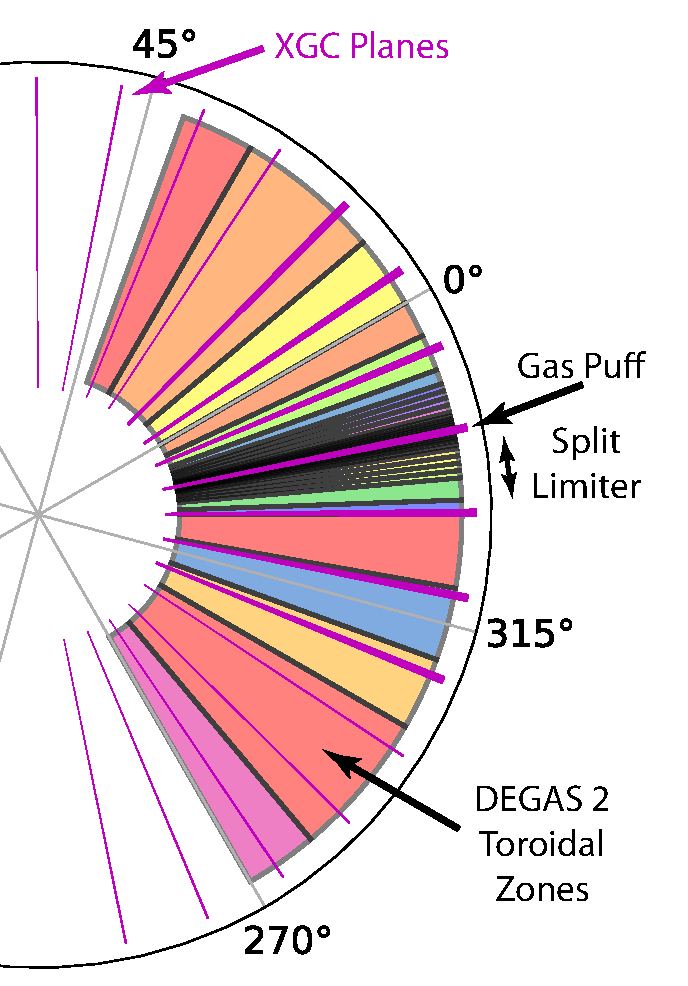
\includegraphics[width=4in]{phi_values_annotated.pdf}
    \caption{Schematic depiction of the toroidal discretizations in
      XGC and DEGAS 2.  The magenta lines correspond to the 16 XGC toroidal
      planes; the thicker ones correspond to the planes used in the
      DEGAS 2 model.  The colored sections represent the DEGAS 2
      toroidal zones,
      corresponding to the values in {\tt phi\_values.txt}.
      The $10^{\circ}$ slices at either end represent
      the toroidal boundaries for the problem; ``mirror'' boundary
      conditions are applied here.  By design, the location of the
      gas nozzle is chosen to coincide with one of the XGC planes.
      The colors of the sections have no particular meaning.}
    \label{phivalues}
  \end{center}
\end{figure}

In the polygon construction section, the limiter sections
and nozzle are solid only over a range of toroidal angles, as is
indicated in {\tt phi\_values.txt} and depicted schematically in
Fig.~\ref{phivalues}.

The toroidal boundary conditions are specified
via the {\tt y\_min\_zone} and {\tt y\_max\_zone} keywords.  We use
{\tt mirror} for both, even though this is not physical.
While an exit boundary
would be preferable here, that is not an option with these commands, 
which
only require the user to specify a ``material''.  Moreover, the
recycling coefficient of that material is hard-coded to unity
in {\tt definegeometry2d}.  Since the path of the camera chords extends
in both directions well away from the gas source, we do not expect
these boundary conditions to affect the results.

{\tt definegeometry2d} does not need to be recompiled, assuming
that {\tt cmodgpi\_camera4.web} remains as {\tt usr2ddetector.web}:

\begin{verbatim}
definegeometry2d XGC_GPI_19_ex/xgc_gpi_19_dg3d.in
\end{verbatim}
Note that this takes significantly longer to run than the 2-D
case, perhaps
4 - 5 hours.

Even though the triangulation is the same as in 2-D, the
associated zone numbers differ, as was noted
above.  Consequently, we
label the polygon netCDF file with ``3d'' and,
thus, the {\tt Triangle} files as well:

\begin{verbatim}
poly_to_tri XGC_GPI_19_ex/gpi_poly_3d.nc
\end{verbatim}


\section{Plasma Setup}

\subsection{Interpolation of XGC Data in the Poloidal Plane}
\label{meshinterp}

The first step in setting up the plasma background for DEGAS 2 is
to interpolate the XGC plasma data
at each of its toroidal planes from its triangular mesh to
the one constructed with {\tt definegeometry2d}.  This is done
with the Python script {\tt xgc1\_gpi\_plasma\_v6.py}.  The script
requires four arguments on the command line:

\begin{enumerate}
\item The directory containing the {\tt H5\_files} directory,
  which in turn has the XGC plasma files.  Since there may be hundreds
  of these files, placing them in a subdirectory is convenient.
\item The name of the XGC plasma file to be processed; this represents
  a single XGC time slice.  Note that these are XGC1's {\tt f3d} output
  files and are produced in {\tt binpack} format with a {\tt .bp}
  extension.  To simplify the task of working with them in Python, they
  have been converted to HDF5 format using the {\tt bp2h5} utility.  The
  integer between the {\tt f3d} and {\tt h5} in the file name is the
  XGC output file number.
  \begin{itemize}
    \item In this run, the XGC variables {\tt sml\_dt} = $9.4 \times 10^{-8}$ s
    and {\tt diag\_3d\_period} = 2 (by default this is equal to the input
    parameter {\tt diag\_1d\_period}) so that each file corresponds to
    $1.88 \times 10^{-7}$ s.
    \item This run, {\tt ti267\_cmod\_IP\_08}, had 484 output files,
    corresponding to 968 total
    XGC steps.
    \item Since the plasma variations over the first 100 files are
      small, the synthetic diagnostic is started at file number 101,
      with file 100 used for initializing the neutral distribution,
      see Sec. XX.
    \end{itemize}
  \item The directory and root file name for the target triangulation onto
    which the XGC data will be interpolated; the script will add {\tt .ele}
    and {\tt .node} to the root file name.
  \item The directory to be used for the output text files.
  \end{enumerate}

  For this example,
\begin{verbatim}
XGC_GPI_19_ex/xgc1_gpi_plasma_v6.py XGC_GPI_19_ex/ xgc.f3d.00100.h5 
         XGC_GPI_19_ex/gpi_poly_2d XGC_GPI_19_ex/
\end{verbatim}

The script loads the XGC's full triangular mesh via the {\tt xgc.py} module
(provided as part of this example).  The target triangulation for DEGAS 2
is then read in from the {\tt .ele}
and {\tt .node} files.  Python and NumPy tools are then used to set
up the interpolation of the node-based XGC data onto the triangle centers,
as is required by DEGAS 2 (all quantities are constant over a triangle / zone).
This yields a set of ``barycentric coordinates''
that can then be used to perform the interpolation from the XGC mesh to
DEGAS 2 mesh in a single expression.

The script reads in the requisite XGC plasma data from the file and
then carries out the interpolations with these adaptations:
\begin{itemize}
\item The ion density is set equal to the electron density.
\item The minimum density is $10^{15}$ m$^{-3}$.
  \item For both the electrons and the ions, an average temperature is computed via:
\begin{equation}
  T = \frac{2}{3}(E_{\parallel} + T_{\perp}
  - \frac{1}{2} m v_{\parallel}^{2}),
\end{equation}
where $E_{\parallel}$ for electrons is {\tt e\_E\_para} in the {\tt f3d} file, likewise
{\tt e\_T\_perp} $\rightarrow T_{\perp}$ and {\tt e\_u\_para} $\rightarrow v_{\parallel}$.
Analogous associations are made for ions.
\item The minimum temperature is 1 eV.
  \item For the ions, the parallel velocity is also written out for use in the
    DEGAS 2 simulations.
  \item To get axisymmetric values for all plasma parameters, we average over
    all toroidal planes.
  \end{itemize}

For this XGC run (and all of the others considered in the development of
the synthetic diagnostic), {\tt sml\_wedge\_n} = 2 so that the 16 toroidal
planes in the file occupy only half of the torus and each toroidal division
is $11.25^{\circ}$ wide; see Fig.~\ref{phivalues}.  
Only seven of the XGC planes are needed
to span the DEGAS 2 zones crossed by the camera view.
The mid-point of these planes is aligned with the
gas nozzle at $\phi = 18.48^{\circ}$.  Arbitrarily, we take XGC plane
number five as the first of the seven planes, going clockwise in the figure.
Separate files are written out for each toroidal plane,
with the plane number incorporated into the file name,
e.g., {\tt plasma\_file\_3.txt}.  The
plasma data are written out in {\tt defineback}'s ``Tabular Format''.
In principle, other formats
can be used if appropriate modifications are made to the 
{\tt get\_n\_t} routine.  

An eighth file, {\tt plasma\_file\_axi.txt},
contains the axisymmetric values in the same format.  A key
difference between this and the other files is that the minimum
density and temperature are reduced to zero.
Since negative axisymmetric plasma data are extremely unlikely,
we do not foresee these minima being enforced in DEGAS 2
triangles that overlap XGC nodes.  Consequently, we will
subsequently use the appearance of zero values in this file
to identify triangles that are outside the XGC mesh.  Some other
more direct mechanism for labeling these triangles, e.g.,
in a separate file, could
in principle be developed should the need arise.

\subsection{Field Line Interpolation}
\label{fieldline}

Were the DEGAS 2 and XGC toroidal discretizations identical,
constructing the DEGAS 2 plasma background from the files
written in the previous step would be trivial.  However,
the requirements of the algorithms in the two codes
are fundamentally different and, thus, so are the toroidal
grids.  To map between the two, we interpolate the
data along a field line.  The fundamental physical
principle is that the variations of the plasma parameters
along a field line should be much smaller than those
in the directions perpendicular to it.

Initial treatments did exactly this.  However, in one
NSTX simulation, the XGC data exhibited greater density
variations along a flux surface than along a field line,
invalidating the simple procedure.  The solution is
to instead interpolate the difference between the local
values and the axisymmetric one, then add the axisymmetric
value back.

The fundamental equation used for field line
following is:
\begin{equation}
  \frac{d \ell}{B} = \frac{dx}{B_{x}} = \frac{dy}{B_{y}}
  = \frac{dz}{B_{z}}.
\end{equation}
Or, in cylindrical coordinates:
\begin{equation}
  \frac{dR}{B_{R}} = \frac{dZ}{B_{Z}} = \frac{R d \phi}{B_{\phi}}.
\end{equation}
This leads us to the actual expressions for integration
along a field line:
\begin{eqnarray}
  \frac{dR}{d \phi} & = & R \frac{B_{R}}{B_{\phi}}, \label{Rphi} \\
  \frac{dZ}{d \phi} & = & R \frac{B_{Z}}{B_{\phi}}.
                          \label{Zphi}
\end{eqnarray}

The magnetic field line structure is derived from the
EFIT equilibrium.  First, the poloidal flux and
other data are fit with spline functions by
subroutine {\tt init\_psi\_interp} in
{\tt psiinterp.web}.  This routine calls
subroutine {\tt test\_interp} upon completion
to compare spline fits with the actual values of
the equilibrium quantities.  Errors in the
spline fits are computed, although no feedback 
is provided to the user.  These should be examined
in cases exhibiting unexpected behavior.
The spline fits form the basis of subroutine
{\tt bvec\_interp}, which returns the magnetic
field vector at the input $R$ and $Z$.

Subroutine {\tt follow\_field}, also in {\tt psiinterp.web},
uses Eqns.~(\ref{Rphi}) and (\ref{Zphi}) to take a small
step along a field line through an input range of
toroidal angle, $\Delta \phi$.  The subroutine
uses a Runge-Kutta scheme of first, second or fourth
order, as determined from its first argument.
For this application, second order is used; this is
specified via the {\tt rk\_order} macro in the
preamble of {\tt xgc1\_gpi.web}.  A detailed
convergence test was performed for all three
orders, examining the scaling of the errors
with the step size.
The first and second order integrations
scaled as expected; the fourth order did not.
Integrations over a long distance, 10 times
around the torus, confirmed these findings.

Note that the experimental GPI systems are designed for a
particular orientation of the magnetic field line, as well
as being optimized for a specific field line pitch.  Since
the geometry of these simulations mimic that experimental
configuration, the user needs to ensure that field line
direction used in the XGC run is the same as in the experiment,
or at least anti-parallel to it.

The relative arrangements of the XGC toroidal planes,
the DEGAS 2 toroidal zone centers, and the boundaries
of the problem, both toroidally and vertically, lead
to three different situations, as is depicted in
Fig.~\ref{interpolation}.

\begin{figure}
  \begin{center}
    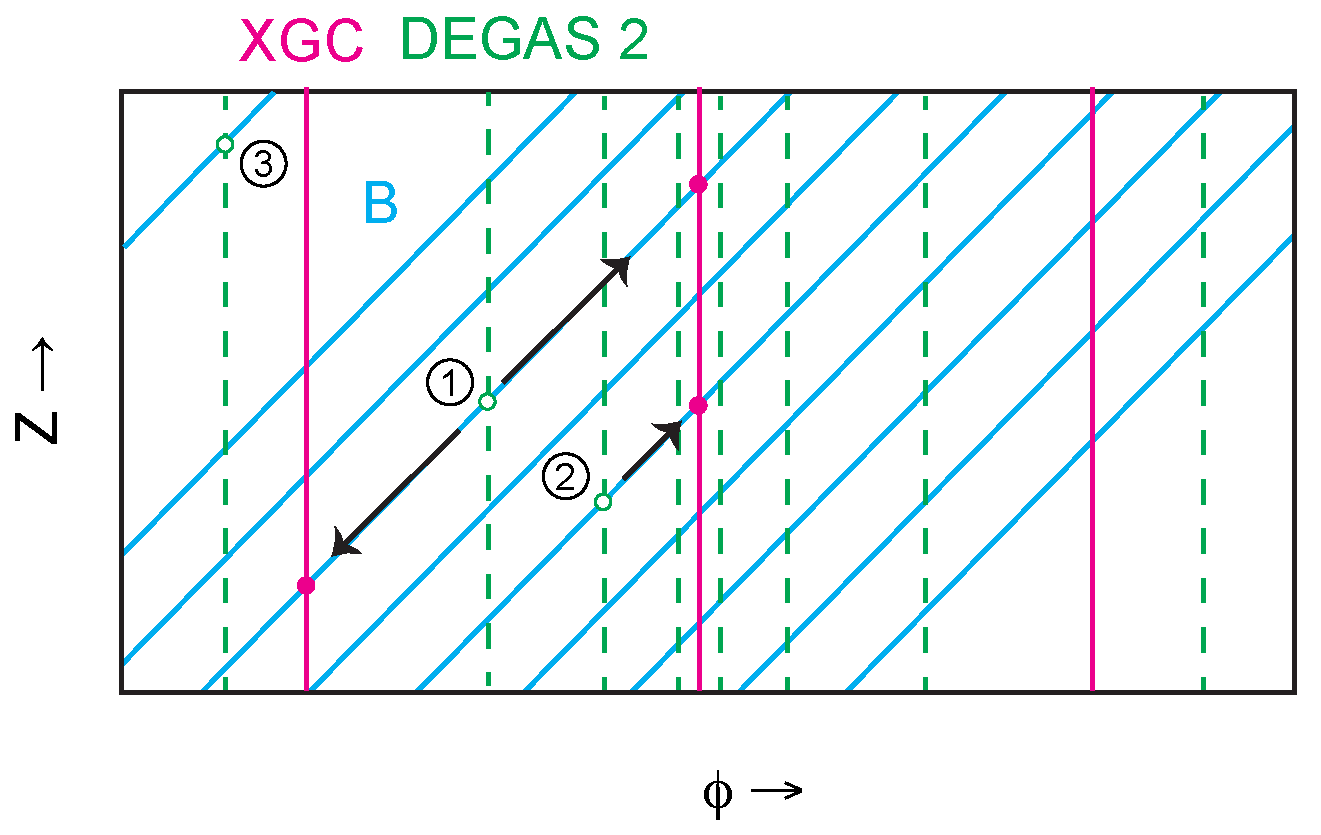
\includegraphics[width=4in]{field_line_interpolation.pdf}
    \caption{Schematic depiction the field line interpolation
      scheme.  The magenta lines represent the XGC toroidal planes.
      The dashed green lines represent the centers of the
      DEGAS 2 toroidal divisions.  The blue lines represent the
    local magnetic field lines.}
    \label{interpolation}
  \end{center}
\end{figure}

\begin{enumerate}
\item Integration in both directions remains within
  the bounds of XGC mesh subset, yielding two XGC data
  values and distances to both $\Rightarrow$ we can
  legitimately interpolate between the two.
\item Integration remains within the box in only one direction.
  Given the notion that plasma parameters, including
  those in ``blobs'', should be roughly constant along
  field lines and that our interpolation distances
  short compared with the parallel connection length,
  we just use the plasma value that we have and use
  it directly.
\item Integration misses the XGC planes in both directions.
  We use the axisymmetric value in this case.
\end{enumerate}

Once the geometry has been set up, the required interpolation
factors for each DEGAS 2 zone can be determined and will not
change.  Hence, we created the XGC interpolation class,
{\tt xgc1interp.hweb}, to hold that information in a
netCDF file; the constituent arrays are documented
at the end of the file.  Once this file has been
created, it can be read in when processing
subsequent time steps, saving considerable time.

\subsection{\tt defineback}

The {\tt get\_n\_t} subroutine for the synthetic GPI
example is in {\tt xgc1\_gpi.hweb} (included with the
DEGAS 2 distribution), which should be
copied to {\tt usr2dplasma.web} and compiled into
{\tt defineback}.
Note that this routine relies on the ``XGC1 interpolation''
class ({\tt xgc1interp.hweb} and {\tt xi\_common} in
the code).  Since this is presently the only invocation
of this class in DEGAS 2 and since the {\tt Makefile.depends}
file generally does not contain entries for the (problem
dependent) {\tt usr2dplasma.web} file, the user should
execute \verb+gmake depend+ in the {\tt src} directory
before compiling {\tt defineback}.
As with virtually all
custom {\tt get\_n\_t} subroutines, the argument to the
{\tt plasma\_file} is a string.  In this case, it
consists of the paths to three files:
\begin{enumerate}
\item The list of plasma files generated by the Python
  script, as described above in Sec.~\ref{meshinterp}.
  The format of this list is prescribed at the top of
  {\tt xgc1\_gpi.web}.
\item The EFIT g-file; this should be the same
  one used in Sec.~\ref{efit2dg2d}.
\item The netCDF interpolation file. If this file
  does not yet exist, the interpolation factors will
  be computed along the way and the file written out.
  If it does exist, the factors will be read in from the
  file. For axisymmetric
  simulations (the number of files specified on the
  first line of the plasma file list is $0$), these
  steps are skipped completely, although the subroutine
  still expects to find a string here.
\end{enumerate}
We use generic file names for the plasma file coming from
the Python script so that they will be overwritten with each
time step.  Consequently, the {\tt plasma\_file} argument
also remains the same in going from one XGC time step to
another.  In fact, the only argument in the input file
that varies is {\tt time\_interval}.

\section{Three Approaches to Time Variation}

The contents of the remainder of the input file to
{\tt defineback} depend on the approach used for
handling the time variation in the XGC data.  To
simplify progress through this example, we will
present them in order of increasing complexity.
The designations of the methods is that used in
the
\href{https://doi.org/10.1063/5.0002876}{synthetic GPI paper}.


\subsection{Frozen Plasma Fluctuations (FPF)}

A separate, steady state run is performed on each XGC time slice;
this assumes that the neutral transport time scales are much
faster than those of the plasma turbulence.  This mode of
operation is also the most like that used in experimental
GPI simulations.  Since the DEGAS 2 runs are all
steady state, the {\tt time\_interval} keyword is not
needed in the {\tt defineback} input file, so the
same file, {\tt xgc\_gpi\_19\_db\_ss}
({\tt xgc\_gpi\_19\_db\_3D\_ss} for 3-D)
can be used for
each time slice.  Note that the desired number of flights
is specified here so as to avoid having to manually
set the number in the background netCDF file.

The baseline input file for {\tt tallysetup},
{\tt tally\_xgc\_gpi\_v2.input} is used; it
contains tallies for the avalanche photo-diode
arrays (APD), but not the GPI image.  No
other special considerations are needed for 
{\tt flighttest} or {\tt outputbrowser}.

We do need to set the appropriate macro switches
in {\tt postdetector}.  Edit the lines:
\begin{verbatim}
@m APP NSTX

@#if 0
\end{verbatim}
to read:
\begin{verbatim}
@m APP CMOD_MID

@#if 1
\end{verbatim}
The first enables device specific macro settings
later on, e.g., for specifying the target plane.
The latter toggles between the full camera view
and a subset used for testing.  Note that with the
implementation of compression of the {\tt zone\_frags}
array, the code runs quickly even with a full
frame.  The same {\tt detector\_setup} routine
compiled into {\tt definegeometry2d},
{\tt cmodgpi\_camera4.web}, is
still needed as {\tt usr2ddetector.web}.

The 2-D FPF simulation is sufficiently quick and simple
that we suggest running it as an interactive batch job
with the 
sample batch script, {\tt gpi\_script\_fpf\_int}.
A few details to note:
\begin{itemize}
\item The parallelized {\tt flighttest} executable
  has been renamed {\tt flighttest\_mpi} to avoid
  successive recompiling to switch between scalar
  and parallel versions.
\item The script assumes that the {\tt Camera\_FPF}
  directory already exists.
\item The short file {\tt a\_no} serves two purposes
  in this script.  First, it provides the ``no'' response
  to force {\tt outputbrowser} to exit its interactive
  mode following its execution of the commands in its
  input file.  Second,
  the prior existence of this file effectively aborts the batch
  job.  As is pointed out in the
  script's comments, doing so prevents
  uncontrolled restarts of the batch job, which can overwrite
  ``good'' output files with problematic ones.  Be sure to
  delete {\tt a\_no} before running this script.
\end{itemize}
For the purposes of these examples, we use
XGC files 301 -- 313 since they contain a relatively large
scale instability that can be easily seen in the GPI images;
we will discuss this further in Sec.~XX on visualization.
The GPI image for each step is generated by {\tt postdetector}
and stored in the {\tt Camera\_FPF} directory, as are
the APD signals.  Note that little use of the latter has
been made to date.  Thirteen steps are used to
demonstrate the integration
over multiple steps described
in the paper to improve statistics (for the time dependent
approach) and to achieve an effective frame rate comparable
to that of the GPI camera.  The resulting image is similar
to that of the individual frames.  The 
{\tt acc\_output} code used for the integration
takes advantage of the same machinery
used for restarts to combine the contents of one
DEGAS 2 output netCDF file with another one from the
same problem; see the premable to {\tt acc\_output}
for additional details.

Once the proper operation of the executables
involved in the batch script has been established,
the executables {\tt defineback}, {\tt outputbrowser},
{\tt postdetector}, and {\tt acc\_output}
can be compiled with \verb+DEBUG = no+.
For {\tt flighttest}, parallelization should be
turned on with \verb+MPI = yes+ and the
\verb+MASTER_SAMPLE+ sample switch should be left with the
default \verb+no+.  The two exceptions to these
guidelines are that {\tt flighttest} must
be run in scalar mode for the Fixed Neutral
Density approach, Sec.~\ref{FND}, and that
\verb+MASTER_SAMPLE+ should be \verb+yes+ for
{\tt flighttest} in the time dependent
case, Sec.~\ref{tdnd}.


\subsection{Fixed Neutral Density (FND)}
\label{FND}

A single steady state run is performed on a representative,
axisymmetric background plasma to obtain a 3-D neutral background
that will be held fixed in time.  With that in hand, the XGC plasma data
for each time step are
read in via {\tt defineback}, just as in the FPF mode.  The
principal difference is that {\tt flighttest} is run in
restart mode with the same number of flights as in
the initial neutral background run. 
Since no additional flights are requested, 
the code's primary loops are bypassed.
In this case, however, all of the light emitting reactions are
set up to be computed via the post-processing estimator.
The emission rates are then appropriate to that particular
time step, but the neutral density is that corresponding to
the initial run.
These runs should be performed with {\tt flighttest}
in serial mode, compiled with \verb+MPI = no+.
The time stepping portion of this method is sufficiently
quick that working in 3-D is practical even for an example
calculation; the procedure for generating it was outlined
in Sec.~\ref{3D}.  See also the dedicated input file,
{\tt degas2\_FND.in}.

In the
\href{https://doi.org/10.1063/5.0002876}{synthetic GPI paper},
the plasma used in producing the fixed neutral
background was taken from a time step in the middle
of the XGC run; this matters since the plasma profiles evolve
during the XGC simulation.  That is not the
case for this much shorter example, so we
simply use the first step from the set that
we will be working with:
\begin{verbatim}
XGC_GPI_19_ex/xgc1_gpi_plasma_v6.py XGC_GPI_19_ex/ xgc.f3d.00301.h5 
XGC_GPI_19_ex/gpi_poly_3d XGC_GPI_19_ex/
\end{verbatim}
As described in Sec.~\ref{meshinterp}, this writes to the output
directory ({\tt XGC\_GPI\_19\_ex} here) a
separate text file for each XGC poloidal plane, plus one with
the axisymmetric values.  To avoid confusion between the
``neutral background'' and the plasma background, we will
henceforth refer to the former as ``NB''.

We only need the axisymmetric file  in producing the NB,
so this initial 
{\tt defineback} input file points to {\tt plasma\_file\_list\_2d.txt}.
It also includes {\tt source\_segment\_iy} keyword
required for 3-D:
\begin{verbatim}
defineback XGC_GPI_19_ex/xgc_gpi_19_db_FND_init
\end{verbatim}
We specify here the target number of flights, $8 \times 10^{6}$,
since manually editing the 3-D background netCDF file is not
all that easy.

The same input (and output) file for {\tt tallysetup} is used
in both the initial NB run
and the subsequent restart steps.  The most relevant difference
between this input file and the ones used with the other synthetic
GPI time stepping methods is that the post-processing estimator
is selected for the {\tt ionize}, {\tt ionize suppress},
{\tt dissociation}, and
{\tt test ion} reaction groups (see the documentation for
\href{tallysetup.pdf#page.3}{tallysetup}).  Doing so violates
the general requirement of using the collision estimator
for the ``test ion'' group, causing an assertion to be
thrown:
\begin{verbatim}
Assertion failed (tallysetup.web): 
    ' Test ions must use collision estimator'=='
\end{verbatim}
The D$_{2}^{+}$ densities are properly computed during the
main loop of {\tt flighttest} so that using the post-processing
estimator to then determine the associated light emission is not
a problem.  The user can either type ``go'' in response to
the assertion (four times), or compile {\tt tallysetup} with
\verb+DEBUG = no+, bypassing the assertion machinery.

The full, 3-D run of {\tt flighttest} with $8 \times 10^{6}$
takes about an hour with $\sim 10^{2}$ cores.  Once complete,
run {\tt postdetector} to generate a corresponding camera
image; we will need this for normalizing the actual time
dependent images.  In a typical application, as in the
\href{https://doi.org/10.1063/5.0002876}{synthetic GPI paper},
one would instead normalize to the
initial, quiescent time slices from XGC.  Since these time
slices are far from quiescent and very similar to each other,
normalizing to the first of them would remove much of the
structure we wish to see.

Rename the output file so that it is not accidentally
overwritten:
\begin{verbatim}
mv degas2_xgc1_cmod_out.nc degas2_xgc1_cmod_NB.nc
\end{verbatim}

Likewise, copy the {\tt postdetector} file to the
output directory to be used for this run (create it
if it does not already exist):
\begin{verbatim}
mv degas2_xgc1_cmod_out_post.nc 
Camera_FND/degas2_xgc1_cmod_out_post_NB.nc
\end{verbatim}

As in the FPF run, the batch job is sufficiently quick that
it can be run interactively, this time on a
single processor, via the script
{\tt gpi\_script\_fpf\_int}.  Some details:
\begin{itemize}
\item Again the file {\tt a\_no} is used to prevent unwanted
  restarts and must be deleted before starting the script.
\item The initial call to {\tt defineback} will take longer
  than subsequent ones since the interpolation file
  (Sec.~\ref{fieldline}) will
  be generated (the run for the
  NB was on an axisymmetric plasma).
\item The same set of XGC files,  301 -- 313, is used.
\item This same {\tt defineback} input file,
  {\tt xgc\_gpi\_19\_db\_3D\_ss} could be used to
  perform a 3-D version of the FPF run.
\item All of these invocations of {\tt flighttest} are
  ``restarts'' with the same number of flights as in
  the NB run.  Consequently, the flag {\tt so\_restart}
  in the background netCDF file needs to be changed from
  its default value of $0$ to $1$.  We do this via a
  few editing commands since {\tt defineback} offers no
  way to do this via its input file.
\item These editing commands could in principle be collapsed
  into a single command via ``pipes'', but have been separated
  to minimize the likelihood of errors.
\item The {\tt postdetector} output files are copied to the
  {\tt Camera\_FND} directory.
\end{itemize}

Note that the {\tt acc\_output} code is {\em not} used
in this application to integrate over frames since the
statistical uncertainty in each frame is exactly the same.
We instead perform simple averages over frames in the
visualization stage, Sec. XX.

\subsection{Time Dependent Neutral Density (TDND)}
\label{tdnd}

We will initially go through this in 2-D, which allows us
use the same input file as the FPF mode:
\begin{verbatim}
cp XGC_GPI_19_ex/degas2_FPF.in degas2.in
\end{verbatim}

Since we already have the geometry file, we can proceed
to set up the snapshot distribution corresponding to the
initial time. First, interpolate the XGC data onto
the DEGAS 2 triangles:
\begin{verbatim}
XGC_GPI_19_ex/xgc1_gpi_plasma_v6.py XGC_GPI_19_ex/ 
    xgc.f3d.00301.h5 XGC_GPI_19_ex/gpi_poly_2d XGC_GPI_19_ex/
\end{verbatim}

Then, run {\tt defineback} with the dedicated input file for
the initialization run:
\begin{verbatim}
defineback XGC_GPI_19_ex/xgc_gpi_19_db_init
\end{verbatim}
Note that we are using the 2-D (axisymmetric) plasma
file here.  The end of the time interval, $1.8802 \times
10^{-7}$ s, will become $t_{0}$ in the subsequent
time dependent run.
The critical keyword in this input file is
{\tt time\_initialization}; this sets the
{\tt so\_time\_initialization} flag in the
\href{classes.pdf#page.31}{sources class} and
in the ``Time Dependence'' section of
\href{degas2_all.pdf#page.28}{the User's Manual}.

Again, because this run uses the same geometry (and
{\tt problemsetup} input file) as the FPF part of the example,
the {\tt tallysetup} netCDF file is the same.  No harm can
come from rerunning {\tt tallysetup} at this point,
however.

\subsubsection{Improving Statistics}
\label{statistics}

The statistics of a time dependent run differ dramatically
from those of steady state simulations.
First note that 
the geometry of these runs has a substantial
plasma-free
volume behind the gas nozzle.
This region is dominated by slow moving molecules or
atoms that do not contribute to the GPI signal.
The principal reason
for including it in the simulations is to provide
a physically realistic
boundary condition for atoms returning from the plasma following
a charge exchange or dissociation event.
A first step in mitigating this problem is to 
reduce the major radius of the vessel wall from
$R=1.0616$ m to
$R=0.98$ m, as was noted in Sec.~\ref{definegeometry2d};
the remaining 5 cm of space behind the gas source is
more than enough to provide the desired boundary condition. For
example, a 3 eV atom (300 K D$_{2}$ molecule or He atom) needs 18
(267) time steps to traverse it.

Another confounding factor is the short mean free
path for atoms heading into the plasma, dropping from an effectively
infinite 25 cm near the nozzle to between 1 and 3 cm around
the separatrix. Since the separatrix is 3.7 cm from the nozzle in this
shot (at the vertical center of the GPI frame), the atoms
must travel more than one mean free path to reach the confined
plasma. But, we need even deeper penetration than this to reach the
regions in which the plasma turbulence is most active.

Two techniques are used to improve the statistics in the region
of interest, i.e., the GPI ``target plane.'' The first, ``suppressed
absorption,'' (also called ``survival biasing'') is commonly used in
DEGAS 2 in connection with the atomic ionization process.
When invoked, the atoms do not undergo discrete ionization events
in which they are completely ionized in a single collision. Rather,
the statistical weight ($=1$ when the particle is
sampled) of the atom
is exponentially reduced along its track with a
rate equal to the ionization
rate. To avoid the tracking of statistically insignificant particles,
a minimum statistical weight is set.
Once that weight is
reached, the decision to either terminate or continue the particle’s
track is made randomly with a $50 \%$ chance for each (``Russian
roulette'').
A typical steady state DEGAS 2 GPI simulation
employs a minimum weight of $10^{-3}$.
In the present case, however, very small
weights will be the norm. To ensure that flights can populate the
inner region as fully as possible, we reduce the minimum weight to
$10^{-7}$. The impact on the run time is modest.  To effect this,
the user needs to set the parameter {\tt WMIN} in {\tt flight.web}:
\begin{verbatim}
@m WMIN const(1.,-7)
\end{verbatim}
Be sure to return this to the default of $10^{-3}$ for use with
more standard problems.

The second technique, importance sampling, is critical for
making the optimal use of the snapshot distribution. By default, the
probability for sampling a particular particle from the
snapshot distribution
is proportional to its statistical weight. Because the cold
molecules and atoms in the vacuum region have undergone little or
no ionization, their statistical weight is comparable to that of newly
sampled gas puff particles. Moreover, the neutral density there is
two or more orders of magnitude larger than in the GPI target
region. Consequently, a direct sample of the snapshot distribution
would be dominated by the cold molecules and atoms in the vacuum
region. Moreover, these particles represent a simple distribution
(thermal molecules or atoms) that can be described adequately
with relatively few particles. In contrast, the particles in which we
are most interested comprise the very kinetic distribution of atoms
resulting from the charge exchange reactions and perhaps containing
complex spatial variations associated with the plasma
turbulence.

The weighting scheme we employ in the importance sampling
is designed to yield a snapshot source
consisting of a radially uniform
number of particles. First, we bin all of the snapshot particles
by major radius in 1 cm wide bins. The inverse of this distribution
then provides the relative weight adjustment factors for the particles
in each bin; these correspond to the
$r_{i,l}$ in Sec.~\ref{final} earlier in this
manual and are computed in
subroutine {\tt set\_snapshot\_source}.
For example, the less-common and lower weight particles
well inside the separatrix will be more heavily weighted,
increasing the likelihood that they will be sampled. The obvious
bias that this introduces is compensated by then
decreasing the statistical
weight carried by these particles during their tracks,
via Eq.~(\ref{statwt}). The
opposite is true of snapshot particles that are sampled at larger
major radius.

To enable this, the user needs to set
the macro flag in {\tt writeback.web}:
\begin{verbatim}
@m GPI_WEIGHTING 1  // Set to 1 for synthetic GPI weighting
\end{verbatim}
This macro also contains code that writes out this binned
distribution to a file called {\tt snapshot\_rel\_wts}
for monitoring after the run.
Again, since this code is specific
for this geometry, its use in other applications may cause
problems; be sure to reset the macro to its default value
of $0$.  Once {\tt defineback} is compiled with this
enabled, the snapshot source will be assigned these
weighting factors.
The file {\tt doflights.web} has a corresponding macro
that writes out the resulting distribution of sampled
particles to {\tt snapshot\_samples}
that can be used to illustrate the effect
of importance sampling.  


Figures~\ref{snapshot1} and \ref{snapshot2} reflect
the snapshot distribution from the initialization run,
as written to {\tt snapshot\_rel\_wts}, and the subsequent
sampling of it, from {\tt snapshot\_samples},
when {\tt flighttest} ran the actual
first time step.  The notebook used to generate
these plots, {\tt XGC\_GPI\_19\_ex\_snapshot\_samples.ipynb},
is included with the example files.

The left plot in
Fig.~\ref{snapshot1}
is nothing more than a pictorial representation of the
sampling process itself; alternatively, it is a plot of the spatial
distribution of the overall neutral probability
distribution function.  Both curves are based on the
total weight in each bin, regardless of species.  The conclusion here
is that the relative weighting and sampling are both working as
intended.

The right plot shows the impact of the relative weighting on the
number of particles (regardless of weight) in each bin; keep in mind
that the key to reducing the variance is to increase the number
of scores, i.e., particles, assuming all of the particles are of
similar weight.
The red curves depict the problematic situation that arises with
weights fixed at 1: most of the particles are D$_{2}$, and the bulk of
these are in an uninteresting region.  The blue curves appear to, and
probably do, sum to roughly a constant; this was the intent of the
relative weight distribution.  The result is a huge increase in the
number of D in the plasma volume, with no change in total weight, and
a reduction in the number of D$_{2}$ in the vacuum region.
Note that we add "1" to the D$_{2}$ curves to allow plotting on a log
scale since their number goes to zero at small $R$.


Figure~\ref{snapshot2} is analogous to the left plot in Fig.~\ref{snapshot1},
but broken down by species.  This demonstrates that the sampling
procedure separately preserves the weight distribution for each
species, even though no explicit provision for doing so has been made.


\begin{figure}
  \begin{center}
    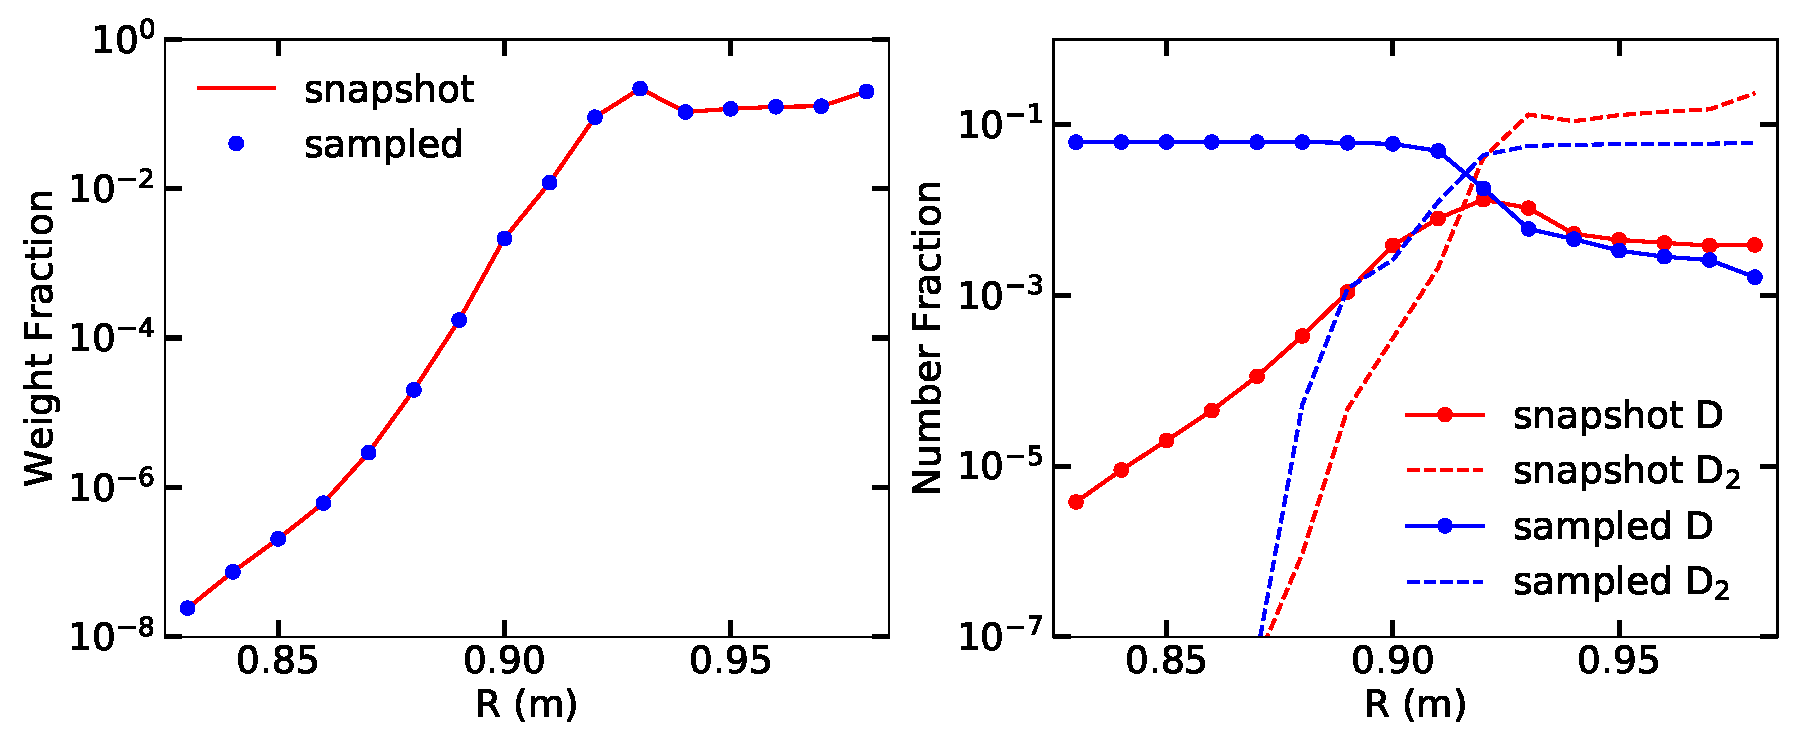
\includegraphics[width=6in]{snapshot_pdfs_1.pdf}
    \caption{Binned probability distribution functions based
      on particle weight (left) and particle number (right).
      Both plots contain lines for the snapshot distribution, as
      contained in the snapshot netCDF file, and for the distribution
      of particles sampled from it prior to tracking in the main code.
      The decoupling of particle number and weight apparent in the
    ``sampled'' plots is the objective of importance sampling.}
    \label{snapshot1}
  \end{center}
\end{figure}

\begin{figure}
  \begin{center}
    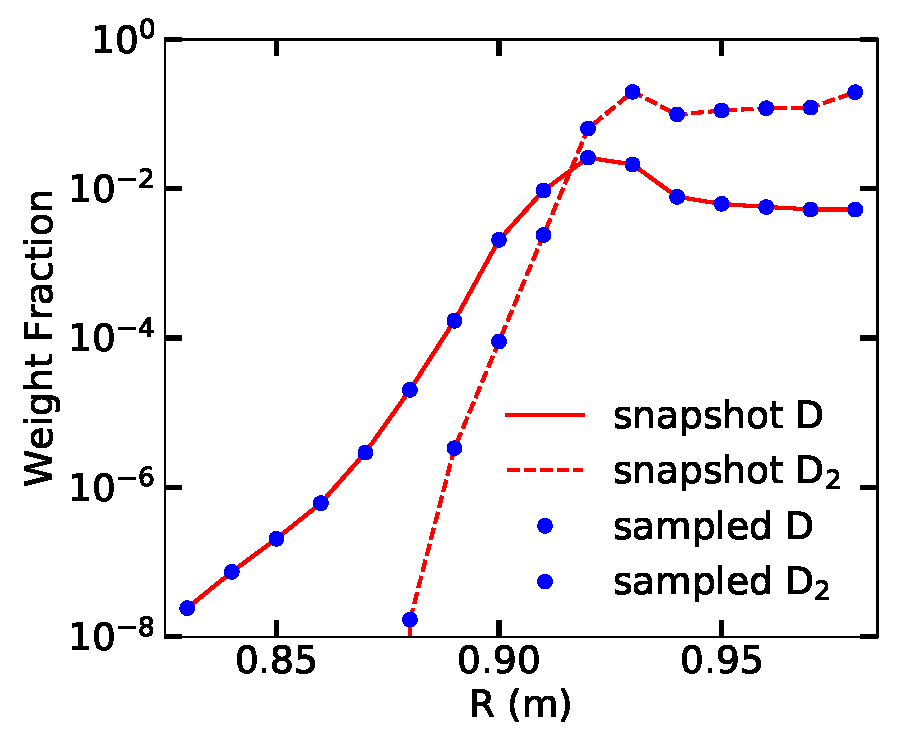
\includegraphics[width=4in]{snapshot_pdfs_2.pdf}
    \caption{Binned probability distribution functions based
      on particle weight, separately for D atoms and
      D$_{2}$ molecules.}
    \label{snapshot2}
  \end{center}
\end{figure}

\subsubsection{Execution}

Due to the large amount of memory occupied by the snapshot
distribution and the associated source, the user should
always run {\tt flighttest} compiled with
\verb+MASTER_SAMPLE = yes+ in the {\tt Makefile.local}
file, even in 2-D.  This will dramatically reduce
the time required for the initial MPI broadcast
to the slaves, as well as the memory they consume.

The batch script for this run, {\tt gpi\_script\_tdnd},
differs from the ones for the FPF and FND methods in
that it:
\begin{itemize}
\item Is intended to be run purely as a batch job,
  i.e, not interactive.
  \begin{itemize}
  \item This is not all that critical for this example,
    which requires about two hours to run.
  \item However, 3-D runs require additional care in
    setting up the processors; see below.
  \item And can take days or even weeks to run the full set of
    XGC time steps.
  \end{itemize}
\item Keeps track of the physical time step, needed for the
  {\tt defineback} input file.
  \begin{itemize}
  \item The \verb+T_ZERO+ set at the top of the script is the
    starting time of the run, representing the end of the
    initialization time step.
  \item Consequently, \verb+T_END+ is initialized to this
    same value; at this point, this is also the time associated
    with the snapshot particles from the initialization run.
  \item At the beginning of a time step, \verb+T_START+ is
    set to \verb+T_END+,
  \item Then \verb+T_END+ is computed from \verb+T_ZERO+, the
    time step size, \verb+DT+, and the step number, \verb+INT_STEP+,
    which is read from the file name.
  \item Note that in this case, we subtract 300 from the step number
    since the first file is for step number 301.
  \item The values of \verb+T_START+ and \verb+T_END+ are written
    into the {\tt defineback} input file via a {\tt sed} command
    which operates on a ``base'' version of the input file,
    {\tt xgc\_gpi\_19\_db\_base}.
    \end{itemize}
\item Compiles diagnostic information on the snapshot
  distribution and on the sampling thereof.
  \begin{itemize}
  \item These files are as described above in Sec.~\ref{statistics}.
  \item But, are concatenated into a single file of the same
    name in the {\tt Camera\_TDND} directory with the step number
    separating each section of the output.
  \end{itemize}
\item The number of particles in each snapshot file is compiled
  in the file {\tt snap\_flights.txt} in the
  {\tt Camera\_TDND} directory.
\item As in the FPF run, the final section of the script integrates
  the output over 13 time steps using {\tt base\_xgc1\_cmod\_out.nc}
  to contain the intermediate output.
  \begin{itemize}
  \item One difference is that we also store every thirteenth snapshot
    file, labeled with the step number, in the {\tt Camera\_TDND}
    directory as a checkpoint and for post-run analysis.
    \end{itemize}
\end{itemize}

\subsubsection{Restarting}

When running hundreds of XGC time steps in total, one may need to
break them up into multiple batch jobs to stay within the
constraints of the batch system.  The best point to stop a
job is at the end of a ``thirteenth'' step since the script
will automatically have saved a copy of
the last snapshot file, reducing
the likelihood of it being deleted or overwritten.  Otherwise,
one just needs to ensure that the snapshot and base output
netCDF files from the end of the last time step are valid.
The other things one needs to do:
\begin{itemize}
\item Set the step number.
  \begin{itemize}
  \item Namely, modify the list of XGC files
    so that it begins with the next step.  E.g., do something
    like:
\begin{verbatim}
XGC1filelist=`ls -1 $XGC1dir/H5_files/xgc.f3d* | tail -163`
\end{verbatim}
    where the ``163'' was chosen to yield the desired step.
  \end{itemize}
\item Set \verb+T_END+ to the time associated with the particles
  in the snapshot netCDF file.
\item Delete the \verb+a_no+ file, as well as the various
  standard output and error files for the batch script and
  the various executables.
\end{itemize}

Should the job be interrupted in the middle of a step, the user
will need to examine the various files and make whatever
adjustments are needed to allow the batch job to be restarted
from the beginning of that step.


\subsubsection{Differences in 3-D}

The memory and storage requirements in 3-D are, not surprisingly,
greater than in 2-D.  The use of the \verb+MASTER_SAMPLE+
option minimizes the load on the slave processes.  In the
original set of TDND runs, extra steps were taken to
ensure that the master process had access to adequate
memory.  First, the script \verb+gen_host_file+ (included
in the example directory) was developed to provide
detailed control over the cores on the master node.
In particular, this script removes 5 cores from the allocated
list on that node so that the memory associated with those
cores can be utilized by the master process.  Accordingly,
the variable \verb+NPROCS+ in the batch script needs to
be 5 smaller than the number of cores requested by the
\verb+SBATCH+ command at the top of the script.  The name
of the file created by \verb+gen_host_file+ is
passed on to {\tt mpirun} via its {\tt hostfile}
argument.  E.g.,
\begin{verbatim}
HOST_FILE_NAME=`gen_host_file`
ARGS="--hostfile "$HOST_FILE_NAME
\end{verbatim}

\section{Visualization and Post-Processing}

The first and simplest visualization of the camera frames
produced by post-detector is demonstrated in the
three Jupyter notebooks included in the example,
one for each approach: {\tt XGC\_GPI\_19\_ex\_FPF.ipynb},
etc.  These include overlaid surfaces representing the
separatrix and XGC's outer boundary.  The movies
can be written to an mp4 file by using the
{\tt save} command of the {\tt matplotlib.animation}
package.  Similar steps can be taken to generate
an analogous movie from the XGC output files,
as in the
\href{https://doi.org/10.1063/5.0002876}{synthetic GPI paper}.

The quantities used to characterize the turbulence,
auto-correlation time, correlation lengths, etc., should
be computed from these frames using the exact
same methods that are applied to the experimental
data.  Doing so ensures an ``apples-to-apples''
comparison.









\tableofcontents

\end{document}